
%----------------------------------------------------------------------------------------
%	PACKAGES AND OTHER DOCUMENT CONFIGURATIONS
%----------------------------------------------------------------------------------------

\documentclass[12pt]{article}

\usepackage[T1]{fontenc}
\linespread{1.02} % A little extra line spread is better for the Palatino font

\usepackage{lipsum} % Used for inserting dummy 'Lorem ipsum' text into the template
\usepackage{amsfonts, amsmath, amsthm, amssymb} % For math fonts, symbols and environments
\usepackage{graphicx} % Required for including images
\usepackage{booktabs} % Top and bottom rules for table
\usepackage{wrapfig} % Allows in-line images
\usepackage[labelfont=bf]{caption} % Make figure numbering in captions bold
\usepackage[top=1in,bottom=1in,left=1in,right=1in]{geometry} % Reduce the size of the margin
\usepackage{textgreek}
\usepackage{gensymb}
\usepackage{marvosym}
\usepackage[font=small,skip=0pt]{caption}

% have clickable links in table of contents and potentially references but i am not there yet
\usepackage{color}
\usepackage{hyperref}
\hypersetup{
    colorlinks=true, % make the links colored
    linkcolor=blue, % color TOC links in blue
    urlcolor=red, % color URLs in red
    linktoc=page, % 'all' will create links for everything in the TOC
    citecolor=cyan
}

\definecolor{orange}{RGB}{255, 165, 0}

\usepackage[utf8]{inputenc}
\usepackage[english]{babel}
\usepackage{fancyhdr}
\usepackage{lastpage}

\usepackage{floatrow}%positioning of captions

\usepackage[font=small,labelfont=bf]{caption}
\usepackage[numbers,sort&compress]{natbib}% hyphenate references 

\DeclareCaptionFont{tiny}{\scriptsize}% declare how large figure captions are. 



\pagenumbering{roman} %type of page numbering you want

\hyphenation{ionto-pho-re-tic iso-tro-pic fortran} % Specifies custom hyphenation points for words or words that shouldn't be hyphenated at all

\begin{document}


%----------------------------------------------------------------------------------------
%	TITLE PAGE
%----------------------------------------------------------------------------------------


%titlepage
\setcounter{page}{0} % no page number on page
\begin{center}
    \centerline{
    
\includegraphics[scale=0.2]{./Figures/northwestern-university-seal-logo.png}}
    \vspace{5cm}
%Thesis title
    {\uppercase{\Large Determining the mechanisms by which natural genetic variation in {\it Caenorhabditis~elegans} contribute to phenotypic variability in response to topoisomerase II poisons\par}}
    \vspace{3cm}
%Author's name
    {\Large {\bf Stefan Zdraljevic}\par}
    \vspace{.75cm}
 %Author's name
   {\Large Advisor $-$ Erik C. Andersen, Ph.D.\par}
    \vspace{.5cm}
%Date
    {\Large June 2nd, 2015}

\end{center}
\clearpage



\newpage


%----------------------------------------------------------------------------------------
%	Table of contents
%----------------------------------------------------------------------------------------

\tableofcontents
\setcounter{page}{0}% no page number on page
%\cleardoublepage
\phantomsection
\listoffigures
\newpage

%----------------------------------------------------------------------------------------
%	Summary
%----------------------------------------------------------------------------------------

\section{Summary}
\setcounter{page}{0}
%This is an example citation ~\cite{Tatro2013}.

Individuals in a population vary in their responses to therapeutic interventions to disease. Identifying the genetic determinants and associated molecular mechanisms underlying such phenotypic variation is a crucial step toward the development of personalized treatment regimens. Advancing personalized medicine has remained difficult because of prohibitive genotyping costs, inability to control environmental conditions, and the polygenic nature of a majority of biomedically relevant traits. To avoid these issues, I will use the tractable model organism {\it Caenorhabditis~elegans} to probe phenotypic variation in response to etoposide and amsacrine, which are two commonly used antineoplastic topoisomerase II poisons. Results from a large-scale phenotyping assay performed on 96 wild {\it C.~elegans} isolates and 359 recombinant inbred lines identified two quantitative trait loci (QTL), on chromosome II and chromosome V, that together explain $\sim$46\% of the phenotypic variance in response to etoposide treatment. Variation in response to amsacrine treatment maps to a QTL in the center of chromosome V that explains $\sim$33\% of the phenotypic variation. Preliminary results from genetic complementation experiments suggest that {\it top-2}, which encodes for a {\it C.~elegans} topoisomerase II, is a causal gene underlying the QTL on chromosome II. The goal of my proposed work is to determine the causal genetic variants underlying the two QTL on chromosome V and any additional causal variants underlying the chromosome II QTL. Identification of causal variants will be achieved by combining classical and quantitative genetics approaches in combination with newly developed CRISPR/Cas9-mediated genome engineering. I will then determine how these variants contribute to differential drug susceptibility through biochemical approaches. The proposed research will be the first attempt to connect molecular changes that result from natural genetic variation to observed phenotypic differences in response to topoisomerase poisons at an organismal level. Importantly, this work has the potential to lead to translatable candidate gene studies in mammalian systems.


\newpage


%----------------------------------------------------------------------------------------
%	SPECIFIC AIMS
%----------------------------------------------------------------------------------------
\pagestyle{fancy}
\section{Specific Aims}
\fancyhf{}
\renewcommand{\footrulewidth}{1pt}
\rfoot{Page \thepage \hspace{1pt} of \pageref*{LastPage}}
\lfoot{Stefan Zdraljevic}
\cfoot{Ph.D. Research Proposal}
\pagenumbering{arabic}

\noindent{\bf AIM 1: Genomic regions underlying QTL will confer resistance to topoisomerase II poisons in an otherwise sensitive genetic background$-$} The size of genomic regions underlying QTL can vary greatly in size and often contain numerous genes with genetic variants ({\it i.e.} candidate genes). The first aim of my project is to reduce the number of candidate genes underlying three QTL that contribute to phenotypic variation in response to the topoisomerase II poisons etoposide and amsacrine. This aim will be accomplished by introgressing the genomic region hypothesized to confer resistance ({\it e.g.} region under QTL) into the sensitive genetic background. Nearly isogenic lines (NILs) that confer resistance will be used to generate NILs with smaller introgressed genomic regions using a speed congenic approach. Successive iterations of this approach in combination with directed gene prioritization will substantially reduce the number of candidate genes to perform functional tests on. 
\vspace{10pt}

\noindent{\bf AIM 2: Specific genetic variants contribute to phenotypic variation in response to topoisomerase II poisons$-$} I will perform the reciprocal hemizygosity test on candidate genes identified in Aim 1 to determine if their function is required to express a phenotype of interest. The reciprocal hemizygosity test is performed by generating two genetically identical reciprocal hybrids that are hemizygous at the gene of interest. Therefore, any differences in the measured phenotype can be attributed to any variants present at the hemizygous locus. Once a gene(s) is found to contribute to topoisomerase II poison sensitivity, I will use CRISPR/Cas9-mediated allele replacement to test individual variants and phenotypic variation. 
\vspace{10pt}

\noindent{\bf AIM 3: The Q797M variant topoisomerase II contributes to sensitivity in response to etoposide treatment$-$} Two tandem single nucleotide variants present in the {\it top-2} gene encode the Q797M missense mutation in strains sensitive to etoposide. This variant is located in the etoposide binding pocket and is predicted to interact with the drug. I hypothesize the Q797M change contributes to differential susceptibility in response to etoposide treatment by stabilizing topoisomerase II-DNA cleavage complexes, which results in increased levels of double stranded breaks throughout the genome. I will directly test this prediction by measuring the half-lives of the topoisomerase II-DNA cleavage complexes encoded by the sensitive and resistant alleles of {\it top-2} in the presence of etoposide.




\newpage


%----------------------------------------------------------------------------------------
%	Background and Significance
%----------------------------------------------------------------------------------------

%=======INSTRUCTIONS FOR SIGNIFICANCE==========



\section{Background and Significance}


\subsection{Significance}


An estimated 40\% of people in the United States will develop cancer at one point in their lives (ACS Surveillance Research, 2015). Of the 1.7 million new people that developed cancer in 2014, 66\% are estimated to survive for at least five years. These statistics underscore the importance of developing new therapeutics as well as developing personalized treatment regimens for cancer. Though incremental steps have been made toward this goal, personalized medicine is still in its infancy. The development of patient-specific regimens largely depends on our ability to obtain accurate genotype and clinical outcome information of many patients that are exposed to the same treatment regimens. Once these data are gathered, statistical associations can be made to correlate a patient's genotype information to his or her treatment outcome. The massively parallel sequencing revolution that has been taking place over the last decade holds promise for identifying the genetic markers associated with diseases such as cancer and our ability to treat them~\cite{Koboldt:2013kw}. However, large-scale studies attempting to link genetic variants with treatment outcomes have largely been unproductive for a number of key reasons. For example, unique variants identified in tumors largely reflect the total number of variants identified in tumors, suggesting that every tumor mostly contains unique variants~\cite{Koboldt:2013kw}. This observation makes it extremely difficult to obtain the required statistical power to identify significant genotype-phenotype associations. The polygenic nature of biomedically relevant traits compounds this issue. Additionally, longitudinal phenotype data are required to link genetic variants to clinical outcomes, which are difficult to obtain for both ethical and practical reasons. As a result, most variants discovered to be associated with outcomes in clinical genome-wide association (GWA) studies do not offer any predictive power for how a patient will respond to treatment~\cite{Park:2012bz}. These and other limitations emphasize the need for novel approaches for identifying variants that predict phenotypic outcomes in clinical settings. I propose using {\it Caenorhabditis~elegans} as a model to identify genetic variants that lead to differential susceptibility to chemotherapeutics. Specifically, I will investigate how natural genetic variation present in the  {\it C.~elegans} population leads to phenotypic variability in responses to chemotherapeutics that alter topoisomerase II function. 
\vspace{-10pt}
\subsection{{\itshape Caenorhabditis~elegans} as a model organism}

Therapeutics used to treat cancer often target conserved cellular processes associated cell division, such as cytoskeleton dynamics, DNA replication, histone modifying enzymes, and growth inducing signaling pathways \cite{Chabner:2005ie}. Conservation of these fundamental processes is highlighted by the  fact that 60-80\% of human genes have homologues present in {\it C.~elegans}~\cite{Kaletta:2006kc}. Importantly, the {\it C.~elegans} genome contains orthologs of pathways that are misregulated in cancer or targeted by therapeutics including components of the receptor tyrosine kinase, Notch, Wnt, TGF-\textbeta , and insulin signaling pathways \cite{Shaye:2011cc}. Classical genetics approaches in {\it C.~elegans} have lead to the characterization of these fundamental pathways and have directed studies in mammalian systems \cite{Wang:2011jy}. These studies have been aided by the numerous genetic, molecular, and cell biological tools available in {\it C.~elegans}. However, much of what we know about {\it C.~elegans} biology stems from the study of a single laboratory strain, N2 \cite{Brenner:1974wn}. Though, as indicated above, research on N2 has been fruitful, much more information can be gained by studying the effects of natural genetic variation in the {\it C.~elegans} population~\cite{GAERTNER:2011gl}. 
\vspace{-10pt}
\subsubsection{Quantitative genetics in \itshape  Caenorhabditis~elegans}

To date, we have identified 124 genome-wide {\it C.~elegans} haplotypes that comprise all of the known genetic diversity in the species \cite{Andersen:2012gm} and unpublished. Each strain contains an average of 85,000 single-nucleotide variants (SNVs) when compared to N2. Importantly, these strains differ in many quantitative traits including growth rate, responses to stress, responses to anthelmintic treatment, food preference, and differential susceptibility to viruses~\cite{Ghosh:2012fza,Ashe:2013bu,Glater:2014jf,Andersen:2015dm,Andersen:2014ec}. These studies are among approximately 20 publications that have found statistically significant associations between specific genetic changes and quantifiable phenotypic differences in {\it C.~elegans}~\cite{GAERTNER:2011gl}. They also highlight our ability to identify causal genes and genetic variants underlying quantitative trait loci (QTL), or genomic regions that contribute to phenotypic differences. Our ability to identify causal genetic variants and genes in {\it C.~elegans} is in stark contrast to the hundreds of GWA studies that have been conducted in humans that typically stop at the identification of QTL~\cite{Tasan:2015er}. Our current inability to link a specific genetic variant to a subtle change in a quantitative phenotype in human studies underscores the importance of using model systems.

\vspace{5pt}

The importance of {\it C.~elegans} as a model organism for quantitative genetics has yet to be fully realized due to lack of scalable assays that can reproducibly identify subtle phenotypic differences in a population. Realizing this, Andersen {\it et al.} established a high-throughput and high-accuracy assay for quantifying differences in fitness related traits~\cite{Andersen:2015dm}. The outline of an updated version of this assay is depicted in \autoref{Phenotyping}. In short, we grow strains for five consecutive generations to eliminate any trans-generational  effects of starvation~\cite{Rechavi:2014ht}. Next, animals are bleach synchronized and embryos are allowed to hatch overnight to the L1 larval stage. The following day, bacterial lysate, which serves as a food source, is added to the growth plates and animals are allowed to grow for two days until they reach the L4 larval stage. Animals are then dispensed to assay plates that contain bacterial lysate, K medium, and a drug (or control) of interest. Sorting is done using the Union Biometrica COPAS large-particle sorter, which identifies L4 animals by size and dispenses three individuals into the prepared assay plate. Four days later, the progeny of the sorted animals are scored using the COPAS large-particle sorter for four traits associated with fitness. These traits include, 1) brood size, 2) animal length, 3) animal optical density, and 4) pharyngeal pumping rate. 
\vspace{5pt}

Using this new approach, we have quantified the phenotypes of 96 wild {\it C.~elegans} isolates and 598 recombinant inbred lines (RILs) exposed to 70 environmental perturbations. The specific goal of my research will be to identify the genetic determinants that contribute to phenotypic variation in response to a subset of chemotherapeutics known to interfere with topoisomerase II function.
\vspace{-10pt}
\subsubsection{Identifying genetic determinants that contribute to phenotypic variation}

We use two approaches to identify genetic loci that contribute to phenotypic variation in a population. The first is a genome-wide association (GWA) approach. The GWA experiments performed in our lab use 96 wild {\it C.~elegans} isolates, identified by Andersen {\it et al.}, that make up all of the known whole-genome haplotypes present in the species~\cite{Andersen:2012gm}. Once phenotype data are generated and processed, we determine if the genotype at a given position in the genome explains phenotypic differences among individuals. Traditional tests for making this type of association include the {\it t}-test, the Wilcoxon rank-sum test, linear regression, or analysis of variance. However, these statistical tests often lead to spurious associations by assuming independence between the genetic marker being tested and the measured phenotype~\cite{Kang:2008bx}. The independence assumption can be violated when studying populations of individuals due to population structure~\cite{Price:2010fc}. For example, if a subset of the assayed population is closely related and susceptible to a topoisomerase poison, then genomic regions corresponding to that subset's relatedness will show up as significantly associated with the susceptibility phenotype. This confounding effect can be greatly reduced by incorporating a {\it strain x strain} relatedness matrix $K$ as a random effect in a linear mixed-model with equation $y = X\beta + Zu +e$, where $y$ is the measured phenotype, $X$ are fixed effects such as the SNP to be tested for association, $Zu$ is the phenotype $y$ corrected for population structure $K$, and $e$ are residual effects \cite{Kang:2008bx}. This methodology was developed for performing GWA on inbred populations, but should be applicable in our system as well. To verify that this is the case, I simulated QTL at every SNV in the genome and tested our ability to identify the QTL. The {\it EMMA} algorithm developed by Kang {\it et al.} outperformed traditional methods such as the Wilcoxon rank-sum test and the {\it t}-test, and other more sophisticated mixed-model approaches like {\it EMMAx} and {\it MLMM} ~\cite{Kang:2010fg,Segura:2012hi}.

\vspace{5pt}

The second approach for identifying QTL uses a panel of recombinant inbred advanced intercross lines (RIAILs) that have been generated from two diverged {\it C.~elegans} strains, N2 and CB4856. These lines were generated by 10 consecutive generations of random pair mating starting with an $F_{3}$ population generated from the three consecutive crosses 1)\,\Male N2\,x\,\Hermaphrodite\,CB4856 and \Male\,CB4856\,x\,\Hermaphrodite\,N2, 2) four possible $F_{1}$ crosses, and 3) four possible $F_{2}$ crosses~\cite{Rockman:2009hb,Andersen:2015dm,Rockman:2008db}. Mating was followed by six generations of selfing to homozygose the genome. Generated RIAILs were then genotyped at 1400 markers across the genomes. Similar to the wild isolates, this reagent set can be used to identify phenotype-genotype associations without the need to correct for population structure. Additionally, this reagent set enables us to identify QTL contributing smaller fractions of phenotypic variation because 500 strains derived from two parental genotypes are being phenotyped. The log of the odds ratio (LOD score) is calculated for every genotyped marker using the formula $LOD = log(1-cor(y,g)^2)/2log(10)$, where $y$ is the measured phenotype and $g$ is the genotype information~\cite{Lander:1995js,Kruglyak:1996uy}. Permutation of the phenotypes and recalculation of LOD scores is performed to set a $5\%$ false discovery rate significance threshold.

\vspace{-5pt}
\subsection{Cellular function of topoisomerases}\label{topos}

The closed double helical structure of DNA makes topoisomerase (TOPO) function essential for all cellular processes~\cite{Champoux:2001cc}. The ability of topoisomerases to cut, exchange strands, and ligate DNA allows for the resolving of numerous topological issues that arise during normal cellular processes such as recombination, transcription, replication, genome condensation, and repair~\cite{Wang:2002hh}. There are two distinct classes of topoisomerases, type I and type II, which cleave one or two strands of DNA, respectively. All topoisomerase enzymes share a catalytic tyrosine residue that mediates DNA scission via a transesterification reaction, however mechanisms that mediate topological relief differ between the different classes~\cite{Vos:2011cra}. 
\vspace{-25pt}
\subsubsection{Type I topoisomerases}\label{TOPO1}

Type I topoisomerases can be further broken up into three distinct classes: Type IA, IB, and the non-ubiquitous IC. Type IA topoisomerase enzymes relax negatively supercoiled DNA that arise behind a transcribing RNA polymerase enzyme during DNA transcription~\cite{Vos:2011cra}. Topoisomerase III, a type IA TOPO, can also resolve hemicatenaned DNA, which occurs as a result of DNA replication, and participates in disentanglement of DNA during recombination~\cite{DiGate:1988ts,Lopez:2005fh}. During DNA relaxation these enzymes pass the intact DNA strand through an enzyme bridged break in the complementary strand that is maintained by a 5'-phosphotyrosyl linkage to the catayltic tyrosine~\cite{Schoeffler:2008dl}.

\vspace{5pt}

Type IB enzymes preferentially target positively supercoiled DNA that form in front of the DNA replication fork and in front of transcribing DNA polymerase \cite{Champoux:2001cc}. Similar to type IA enzymes, type IB TOPOs also bind negatively supercoiled DNA that occurs behind the transcribing RNA polymerase. However, distinct from the type IA mechanism, type IB topoisomerases mediate topological solutions by nicking one strand of DNA and forming a 3'-phosphotyrosyl linkage to the catayltic tyrosine. Positive supercoils are relaxed by rotating the intact strand counterclockwise and negative supercoils are relaxed via clockwise rotation~\cite{Stewart:1998te}. 
\vspace{-10pt}
\subsubsection{Type II topoisomerases}\label{TOPOII}

In contrast to type IA enzymes, type II TOPOs mediate resolution of DNA topological issues via double stranded breaks. As a result, they alter the writhing number of DNA and can alter the linking number by a factor of $\pm$2~\cite{Champoux:2001cc}. Type IIA and IIB have similar functional and mechanistic roles, but type IIB are only found in archaea, plants, bacteria, and algae~\cite{Vos:2011cra}. 

\vspace{5pt}

Two type IIA topoisomerases are present in all organisms from humans (topoisomerase II\textalpha\ and II\textbeta) to {\it Escherichia coli} (gyrase and topoisomerase IV)~\cite{Wang:2002hh}. {\it C.~elegans} and {\it Saccharomyces cerevisiae} only contain one type IIA enzyme, simply referred to as DNA topoisomerase II. The biochemical activity between the human TOPOII\textalpha\ and II\textbeta\,isoforms is indistinguishable as a result of high levels of sequence homology with approximately 70\% identity and 85\% similarity~\cite{Austin:1995ua}. The isoforms differ mostly in the C-terminal regions, which are subject to multiple types of post-translational modification that modulate isoform specific functions~\cite{Linka:2007jo}. Though both enzymes are essential for viability in mammalian systems, only topoisomerase II\textalpha\ is essential for solving DNA entanglements and mediating sister chromatic segregation during mitosis. Due to this essential function during the cell cycle, topoisomerase II\textalpha\ is upregulated 2-3 fold during the G2/M phase of the cell cycle and is the target of numerous chemotherapeutics~\cite{Wu:2013dia}. 

\vspace{5pt}

The catalytic cycle of type IIA topoisomerases involves 1) DNA binding, 2) ATP binding, 3) DNA cleavage, 4) strand passage, 5) religation, and 6) strand release. The gate or "G" DNA strand enters the topoisomerase holoenzyme via the TOPRIM domain and is maintained in the catalytic site by interactions with the C-terminal helix of the winged-helix domain (WHD) and the \textalpha\textbeta\ fold tower domain~\cite{Chang:2013bn,Dong:2007ita}. Lack of specificity in DNA binding is thought to occur due to the atypical interaction of the WHD domain with the phosphate backbone of only one DNA strand ~\cite{Dong:2007ita}. Substantial ($\sim$150\degree) bending of the G-strand DNA, which is mediated by the WHD and the tower domain, occurs prior to the binding of two ATP molecules to the ATPase domain and trapping of the transport (T) DNA strand in the N-gate GHKL domain. ATP hydrolysis of one ATP molecule simultaneously stimulates G-strand cleavage and T-strand passage through the cleaved strand. Cleavage of the G-strand by the catalytic tyrosine creates a four nucleotide overhang and a phosphotyrosyl linkage between the tyrosine and phosphate of the +1 5' nucleotide, referred to as Top2 cleavage complex (Top2cc). DNA religation after strand passage leads to G-strand interaction with the K-loop present in the transducer domain that stimulates secondary ATP hydrolysis and dissociation of product molecules~\cite{Schmidt:2012eu}. Over the course of the past three decades, compounds have been identified to target all stages of the type II topoisomerase catalytic cycle. 
\vspace{-10pt}
\subsubsection{Topoisomerase II poisons $-$ Etoposide and Amsacrine}\label{top2inh}

The two main types of compounds that affect topoisomerase II function are those that inhibit the catalytic activity of the enzyme and those that lead to increased levels of Top2cc, which are often referred to as topoisomerase poisons. Topoisomerase II poisons take advantage of a vulnerable point in the the catalytic cycle just after DNA cleavage when the enzyme is covalently bound to the DNA~\cite{Nitiss:2009kg}. A subset of poisons, including etoposide and amsacrine act by sterically hindering the 3' OH of the recently cleaved -1 nucleotide from performing a nucleophilic attack on the 5'-phosphotyrosyl linkage of the Top2cc~\cite{Wu:2013dia}. The significance of these molecules in treating cancer is underscored by their usage in the clinical setting. For example, etoposide is one of the most commonly used anti-neoplastic compounds and is used in at least 31 different treatment regimens to treat nine different types of cancer, though it is primarily used to treat lung and testicular cancer (http://www.cancerresearchuk.org/). These drugs are often taken in combination therapy with compounds that inhibit other cellular pathways or components such as DNA repair and replication (intercalators and alkylating agents), microtubule dynamics, and cellular signaling and metabolism. Responses to chemotherapeutic intervention remain highly variable among patients, despite the fact that antineoplastic drugs target essential cellular pathways. Much of this variation is likely due to genetic factors that have yet to be identified in many underpowered clinical GWA studies~\cite{Low:2013jw,Huang:2007id}. In addition to differential efficacy, antineoplastic treatments are often associated with a variety of side effects. An extreme example of such side effects is the development of secondary malignancies that occur in response to treatment with etoposide, which occurs in approximately 1\% of patients (http://www.cancerresearchuk.org/). Clinical studies are often underpowered due to the small case and control populations, poorly controlled treatment regimens and electronic record systems, and the genetic architecture underlying a particular trait ({\it e.g.} a rare variant of medium to large effect or many variants of small effect)~\cite{Koboldt:2013kw,Park:2012bz}. 
\vspace{-10pt}
\subsection{Variation in response to topoisomerase II poisons in {\itshape C.~elegans}}\label{preliminary}

Preliminary work aimed at identifying the genetic determinants underlying etoposide and amsacrine sensitivity in {\it C.~elegans} has led to the identification of numerous QTL, three of which are shown in \autoref{LODplot}A-B. These data were generated using the high-throughput phenotyping pipeline for measuring traits associated with animal fitness that is outlined in Appendix \autoref{Phenotyping}. As seen in \autoref{LODplot}, variation in response to etoposide treatment mapped to two main QTL, one that appeared in both linkage and GWAS experiments (Appendix \autoref{GWAS}A) on the right arm of chromosome II and the other to the center of chromosome V. Interestingly, SNVs in the {\it top-2} gene, which underlies the QTL on chromosome II and encodes for one of two topoisomerase II enzymes in {\it C.~elegans}, are most significantly associated with variability in response to etoposide (Appendix \autoref{GWAS}B). The {\it top-2} gene contains four highly correlated missense variants between the laboratory strain N2 and the wild isolate CB4856. Of these variants, three are in the C-terminal domain (CTD - 	E1217A, D1387N, G1419D) and one is predicted to reside in the etoposide drug binding pocket (Q797M) (\autoref{LODplot}C)~\cite{Sanchez:2011jn}. These variants are also present in approximately 35\% of the wild-isolate population and are predictive markers for drug susceptibility (Appendix \autoref{GWAS}). Surprisingly, amsacrine, which is also a topoisomerase II poison does not map to the same location on chromosome II, suggesting that the variants present in {\it top-2} are not affecting normal protein function or expression. However, phenotypic variation in response to amsacrine maps to the center of chromosome V and overlaps the etoposide QTL. It is interesting to note that CB4856 is resistant to amsacrine treatment and sensitive to etoposide, suggesting that the QTL on chromosome V is drug specific.

\begin{figure}[h]
\centering
\captionsetup{font=tiny}
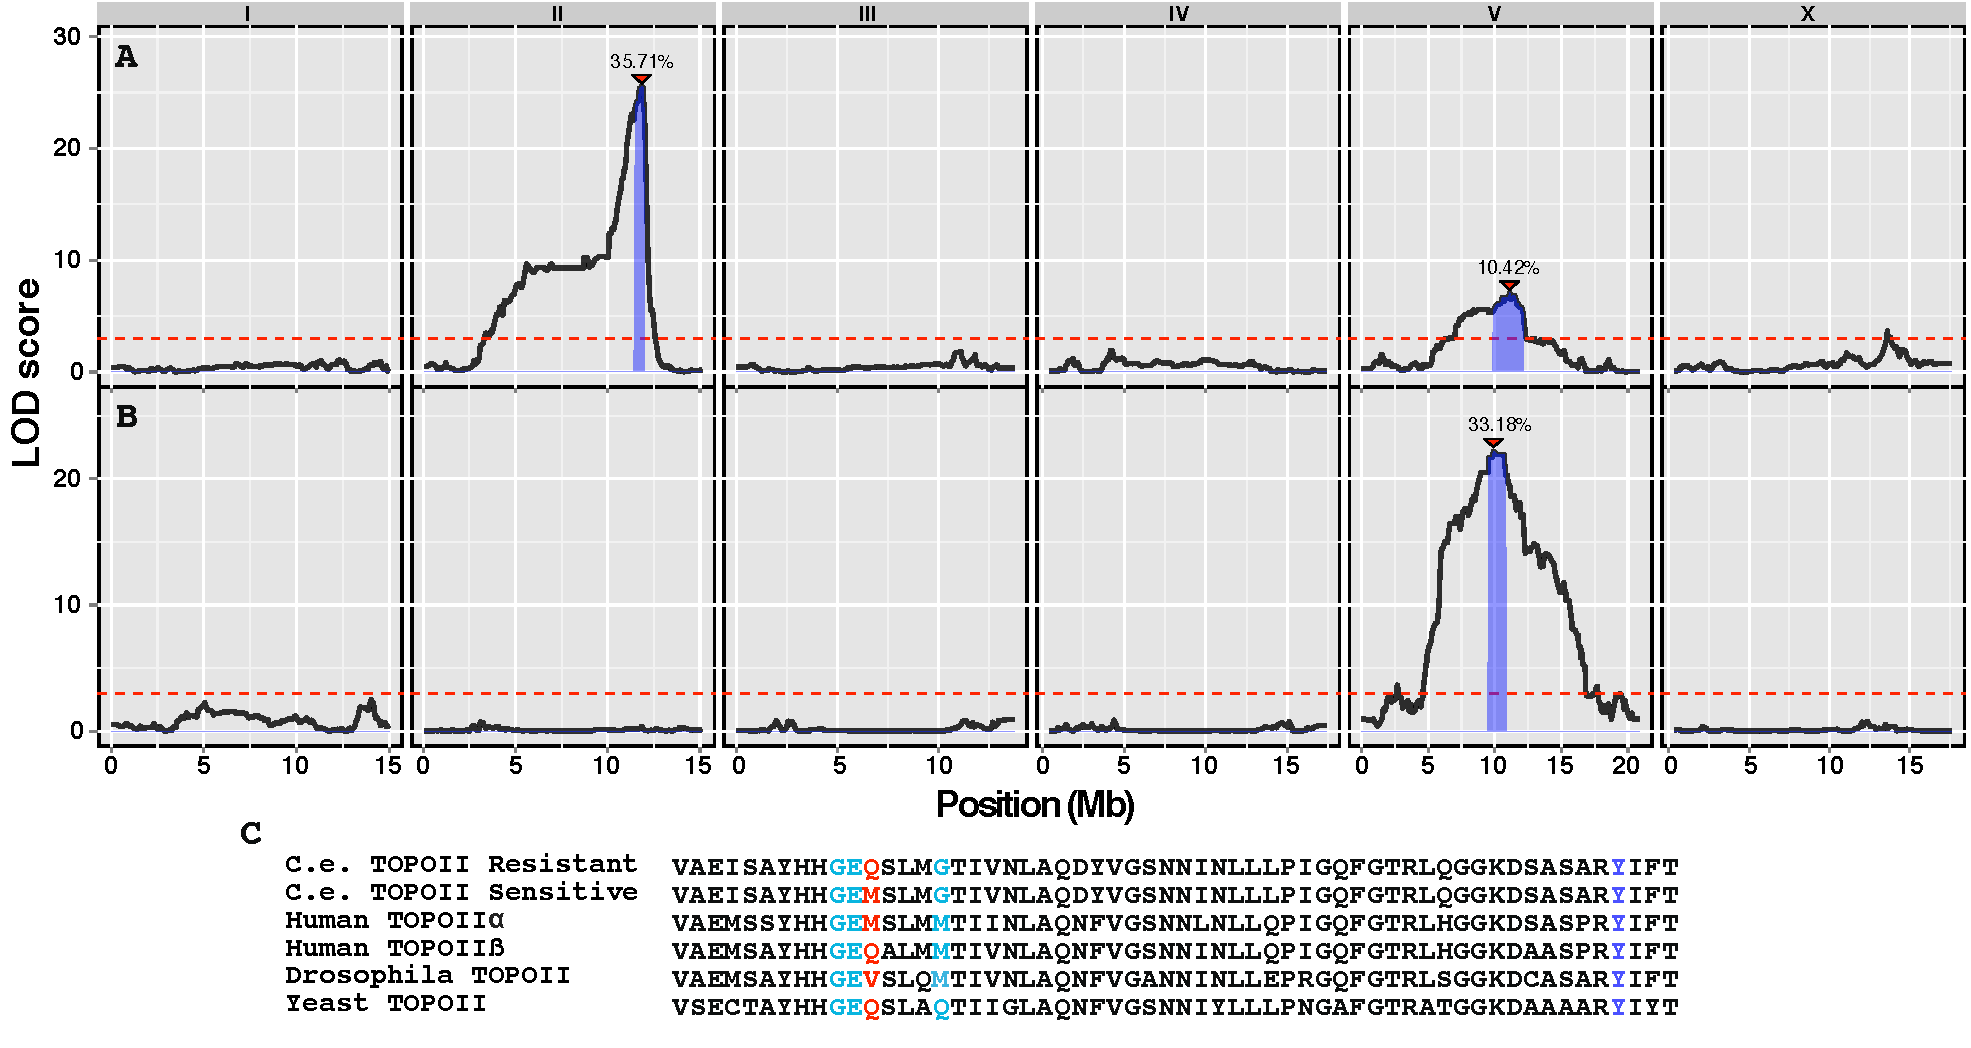
\includegraphics[scale=0.45]{Figures/Figure1.pdf}
\vspace{-5pt}
\caption[LOD plots for TOPOII poisons]{LOD plots showing QTL identified using the RIAIL collection. Blue bars under QTL represent associated confidence intervals. Red triangles correspond to the peak position, with corresponding percentage of phenotypic variance explained by loci directly above. Red dotted line corresponds to a $5\%\,FDR$ threshold. A) Treatment - etoposide, phenotype - brood size and B) Treatment - amsacrine, phenotype - animal size. C) Multiple sequence alignment of different TOPOs. Dark blue is the catalytic tyrosine, which is conserved in all TOPOII proteins. Light blue and red correspond to drug binding pocket. Red is the genetic variant hypothesized to lead to differential susceptibility.}
\label{LODplot}
\end{figure}
\newpage

%--------------------------------------------------------------------------------------------------------------------------------------------------------------------------------
%	Experimental Design and Methods
%--------------------------------------------------------------------------------------------------------------------------------------------------------------------------------
%--------------------------------------------------------------------------------------------------------------------------------------------------------------------------------
%	Experimental Design and Methods
%--------------------------------------------------------------------------------------------------------------------------------------------------------------------------------
%--------------------------------------------------------------------------------------------------------------------------------------------------------------------------------
%	Experimental Design and Methods
%--------------------------------------------------------------------------------------------------------------------------------------------------------------------------------
%--------------------------------------------------------------------------------------------------------------------------------------------------------------------------------
%	Experimental Design and Methods
%--------------------------------------------------------------------------------------------------------------------------------------------------------------------------------


\section{Experimental Design and Methods}\label{Methods}

\subsection{Specific Aim 1 $-$ Narrow QTL confidence intervals}\label{Aim1}

Identification of a QTL suggests that there is genetic variation at that locus that is contributing to phenotypic variability. All QTL have an associated confidence interval that ranges in size depending on numerous factors. One of the most important factors that determines the size of a QTL confidence interval in our linkage mapping experiments is the genomic recombination rate~\cite{Kessner:2015hs}. For example, confidence intervals are much smaller on the arms of chromosomes, where recombination rate is higher, than in the center of chromosomes, where recombination rate is lower~\cite{Rockman:2009hb}. Recombination rate plays an important role in linkage mapping because it generates break points where the origin of the recombinants' genome switches between N2 and CB4856. These break points allow us to determine which parental genotype is contributing to the observed phenotypic variation for a given quantitative trait. Similarly, in GWA experiments, recombination plays a key role in breaking up large linkage disequilibrium ($LD$) blocks present in the genome. {\it C.~elegans} has an unusually high level of LD given the observed levels of recombination rate~\cite{Rockman:2009hb}, which is largely due to recent chromosome-wide selective sweeps in the population and a primarily hermaphroditic mating system~\cite{Andersen:2012gm}. An equally important and related factor contributing to interval size is the number of individuals phenotyped, because increasing the number of individuals gives more opportunity to sample different recombinants in linkage mapping and different haplotypes in GWA. The combination of these two factors is why we tend to observe smaller confidence intervals in linkage mapping experiments.

\begin{table}[h]
\caption{QTL Confidence Intervals}
\begin{center}
\begin{tabular}{|| c c c c c c c ||}
\hline
{\bf Drug} & {\bf Chr} & {\bf Left} & {\bf Peak} & {\bf Right} & {\bf Genes} & {\bf Genetic Distance (cM)}\\
\hline\hline
Etoposide & II & 11492171 & 11833729 & 12008179 & 28 & 7.00\\
Etoposide & V & 9903872 & 11114697 & 12125475 & 97 & 13.35\\
Amsacrine & V & 10124453 & 10720948 & 11004172 & 35 & 5.40\\
\hline 
\end{tabular}
\end{center}
\label{default}
\vspace{-15pt}
\label{Intervals}
\end{table}
\vspace{-10pt}

QTL confidence intervals from linkage mapping experiments and the number of genes contained within each are shown in~\autoref{Intervals}. These confidence intervals correspond to QTL in \autoref{LODplot}. The number of genes present in these confidence intervals make it difficult to perform experiments to establish gene causality. However, the etoposide QTL on chromosome II contains a strong candidate gene, {\it top-2}, which encodes a homolog of human topoisomerase II\textalpha. Experiments to establish gene causality for {\it top-2} and other candidate genes are discussed in sections \ref{Aim21} and \ref{Aim22}. Having a strong candidate gene underlying the etoposide chromosome II QTL does not exclude the possibilities that it is not the correct gene or that there are many contributing genes underlying the QTL. I will construct nearly isogenic lines (NILs) to eliminate these possibilities for this QTL and to narrow the confidence intervals associated with both chromosome V QTL.

\vspace{5pt}

NILs are generated by reciprocally introgressing the genomic region defined by a QTL confidence interval from the genetic background with one phenotype into the genetic background of a strain with the alternative phenotype. In our assays, where animals are being subjected to treatment with topoisomerase poisons, the alternate phenotypes are relative susceptibility and resistance. In the case of etoposide treatment, the standard laboratory strain N2 is resistant to treatment and the wild isolate CB4856 is sensitive. This relationship is the same for the QTL on chromosome II and the QTL on chromosome V (\autoref{PxG}A-B). Interestingly, genetic variation underlying the amsacrine QTL on chromosome V has the opposite effect (\autoref{PxG}c) and CB4856 has the resistant phenotype. The difference in effect associated with the QTL on chromosome V suggests that the underlying variants are contributing to phenotypic variability in a drug-specific manner and not a common pathway related to DNA damage. 

\begin{figure}[h]
\captionsetup{font=tiny}
\centering
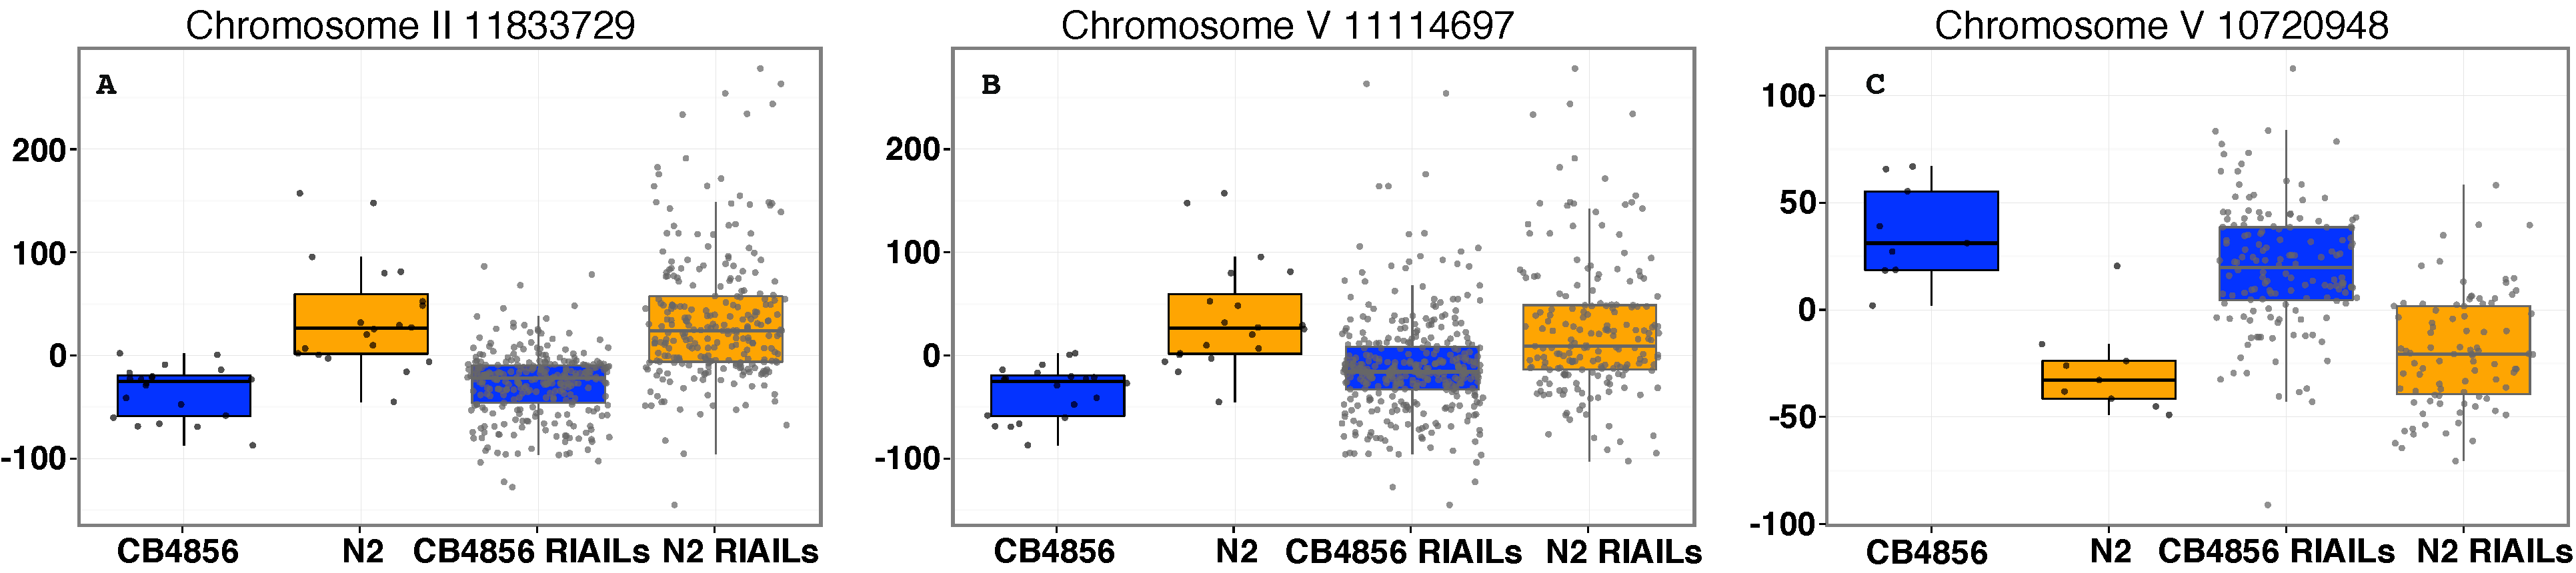
\includegraphics[scale=0.25]{Figures/Figure2.pdf}

\caption[Phenotype by genotype splits for QTL]{Phenotypes from linkage mapping split by genotype at the genomic position above corresponding plot. A and B) Phenotype in response to etoposide, C) Phenotype in response to amsacrine. Parental strains CB4856 and N2 were phenotyped in multiple replicates, each point corresponds to a replicate. RIAILs were phenotyped in one replicate and each point corresponds to one RIAIL. RIAILs are grouped and colored by what the parental genotype is at the locus being plotted.}
\label{PxG}
\end{figure}

NILs will first be generated by introgressing the genomic region corresponding to the entire QTL confidence interval. I will generate NILs by crossing a RIAIL that has a continuous parental genotype block overlapping a QTL confidence interval  to CB4856 or N2, depending on the direction of introgression. Insertion or deletion variants (indels) that exist between CB4856 and N2 will be used to verify that recombination did not occur within the genomic region being maintained. Six consecutive generations of back crossing to parental CB4856 or N2 will homogenize the genetic background such that the resulting strain will have the parental genotype in approximately 99\% of the genome and the introgressed region of interest with the opposite genotype. Crosses will be followed by six consecutive generations of hermaphroditic selfing to homozygose any portion of the genome that was not converted to the N2 or CB4856 genotype. Once NILs are generated, I will phenotype them in the presence of etoposide or amsacrine to see if the introgressed genomic region confers the expected phenotype.

\vspace{5pt}

NILs that recapitulate the correct phenotype will be used to generate NILs with smaller introgressed genomic regions through speed congenics~\cite{Wong:2002wc}. The speed congenic approach requires the presence of multiple markers that span the genomic region of interest to identify recombinants ($\sim$100~indels/Mb between CB4856 and N2). The cross design for speed congenics is depicted in \autoref{NILs}. In short, male NILs will be backcrossed to the background genotype to generate heterozygous $F_{1}$ animals. Heterozygote males will then be backcrossed to the parental strain to generate $F_{2}$ animals of unknown genotype ({\it e.g.} recombinant or parental). Single $F_{2}$ hermaphrodites will be placed in 96-well plates and allowed to self. Half of the $F_{3}$ progeny will be used to genotype indels across the interval by PCR and the other half will be saved to isolate positive recombinants. $F_{2}$ progeny are added to the wells because we expect a fraction of them to be recombinants, therefore enabling easier recovery of recombinants in subsequent generations. By genotyping numerous markers across a genomic region, we expect to identify recombinants with breakpoints in different locations, thus generating a panel of NIL strains that have the introgressed genotype tiling across the confidence interval. To obtain recombinants that have sufficiently broken up the interval on chromosome V and II, I will need to genotype approximately 200 $F_{3}$ progeny ({\it i.e.} $\sim$2~recombinants/cM). These NILs will then be phenotyped to see which smaller genomic region confers the desired phenotype. 

\vspace{5pt}
{\bf Progress: }I have already generated NILs that span the entire confidence interval for the etoposide chromosome II QTL. Though we have a strong candidate gene underlying this QTL, other variants in this region can be contributing to phenotypic variation. I will phenotype these strains once NILs are generated for the chromosome V peaks, which are currently being generated.

\vspace{5pt}
{\bf Potential issues: }If there are still many candidate genes after successive rounds of NIL generation, we can prioritize genes by looking at any associated annotation or functional data and by looking at the phenotype-genotype correlation of genetic variants present within the confidence interval. The results of such an approach are depicted in \autoref{GWAS}B-C for the phenotypes of the wild isolates in response to etoposide. In short, phenotyped strains are split by the presence of a genetic variant within a confidence interval. Variants with the highest phenotype-genotype correlation are considered to be high priority targets. In the case of etoposide, two out of 28 genes are highly correlated with phenotype (Spearman's $\rho > .5$). One gene is {\it top-2} and the other is the neighboring gene {\it npp-3}, which is expected due to high $LD$ between the two genes. 
\vspace{5pt}

There is the potential that NILs do not recapitulate the expected phenotype. One reason this might occur is due to the RIAIL used as a starting strain for the introgression did not have the expected genotype ({\it i.e.} RIAILs were not whole-genome sequenced). Any discrepancies will be identified when members of the lab generate whole-genome sequence information for the RIAILs. Another reason for NILs might fail to recapitulate the expected phenotype is due to epistasis~\cite{Fisher:2000ta}. This is unlikely because I have performed a test for interacting loci using a pairwise scan from the R/qtl package~\cite{Broman:2009gn}.

\vspace{-5pt}
\subsection{Specific Aim 2 $-$ Establish gene and variant causality}\label{Aim2}

\subsubsection{Gene causality}\label{Aim21}

Many genetic tests can be performed to link a gene product's function with a particular phenotype, thereby establishing that gene as causal. As was stated in a recent review by David Stern, the "gold standard" for providing evidence that genetic variation in a candidate gene is causing phenotypic variation is to perform allele replacement at the candidate locus~\cite{Stern:2014jp}. This approach will be discussed in Section \ref{Aim22}. 

\vspace{5pt}


\begin{figure}[h]
\captionsetup{font=tiny}
\floatbox[{\capbeside\thisfloatsetup{capbesideposition={right,top},capbesidewidth=6cm}}]{figure}[\FBwidth]
{\caption[Establishing {\it top-2} causality]{Establishing {\it top-2} causality. A)~Results from the dominance experiment. Hermaphrodites of N2 and CB4856 were crossed to male N2 reporter strain containing GFP, ensuring all hermaphrodite GFP progeny to be heterozygous. Three GFP positive progeny were exposed to 500~\textmu M etoposide or DMSO and allowed to self over the course of four days. Heterozygous progeny are colored light green and homozygous N2-GFP strains are dark green. B)~Results from the complementation experiment. Male N2 or CB4856 were crossed to hermaphrodite {\it\textDelta top-2}/{\it mIn1} N2 animals that also contain GFP reporters. Three non-GFP hermaphrodite progeny (heterozygous for the parental strain and {\it\textDelta top-2}) were placed in experimental plates and allowed to grow as described above. Knockout heterozygous progeny are labeled gray. Phenotype values from control conditions were regressed out to generate residual values, which are plotted.}\label{DomComp}}
{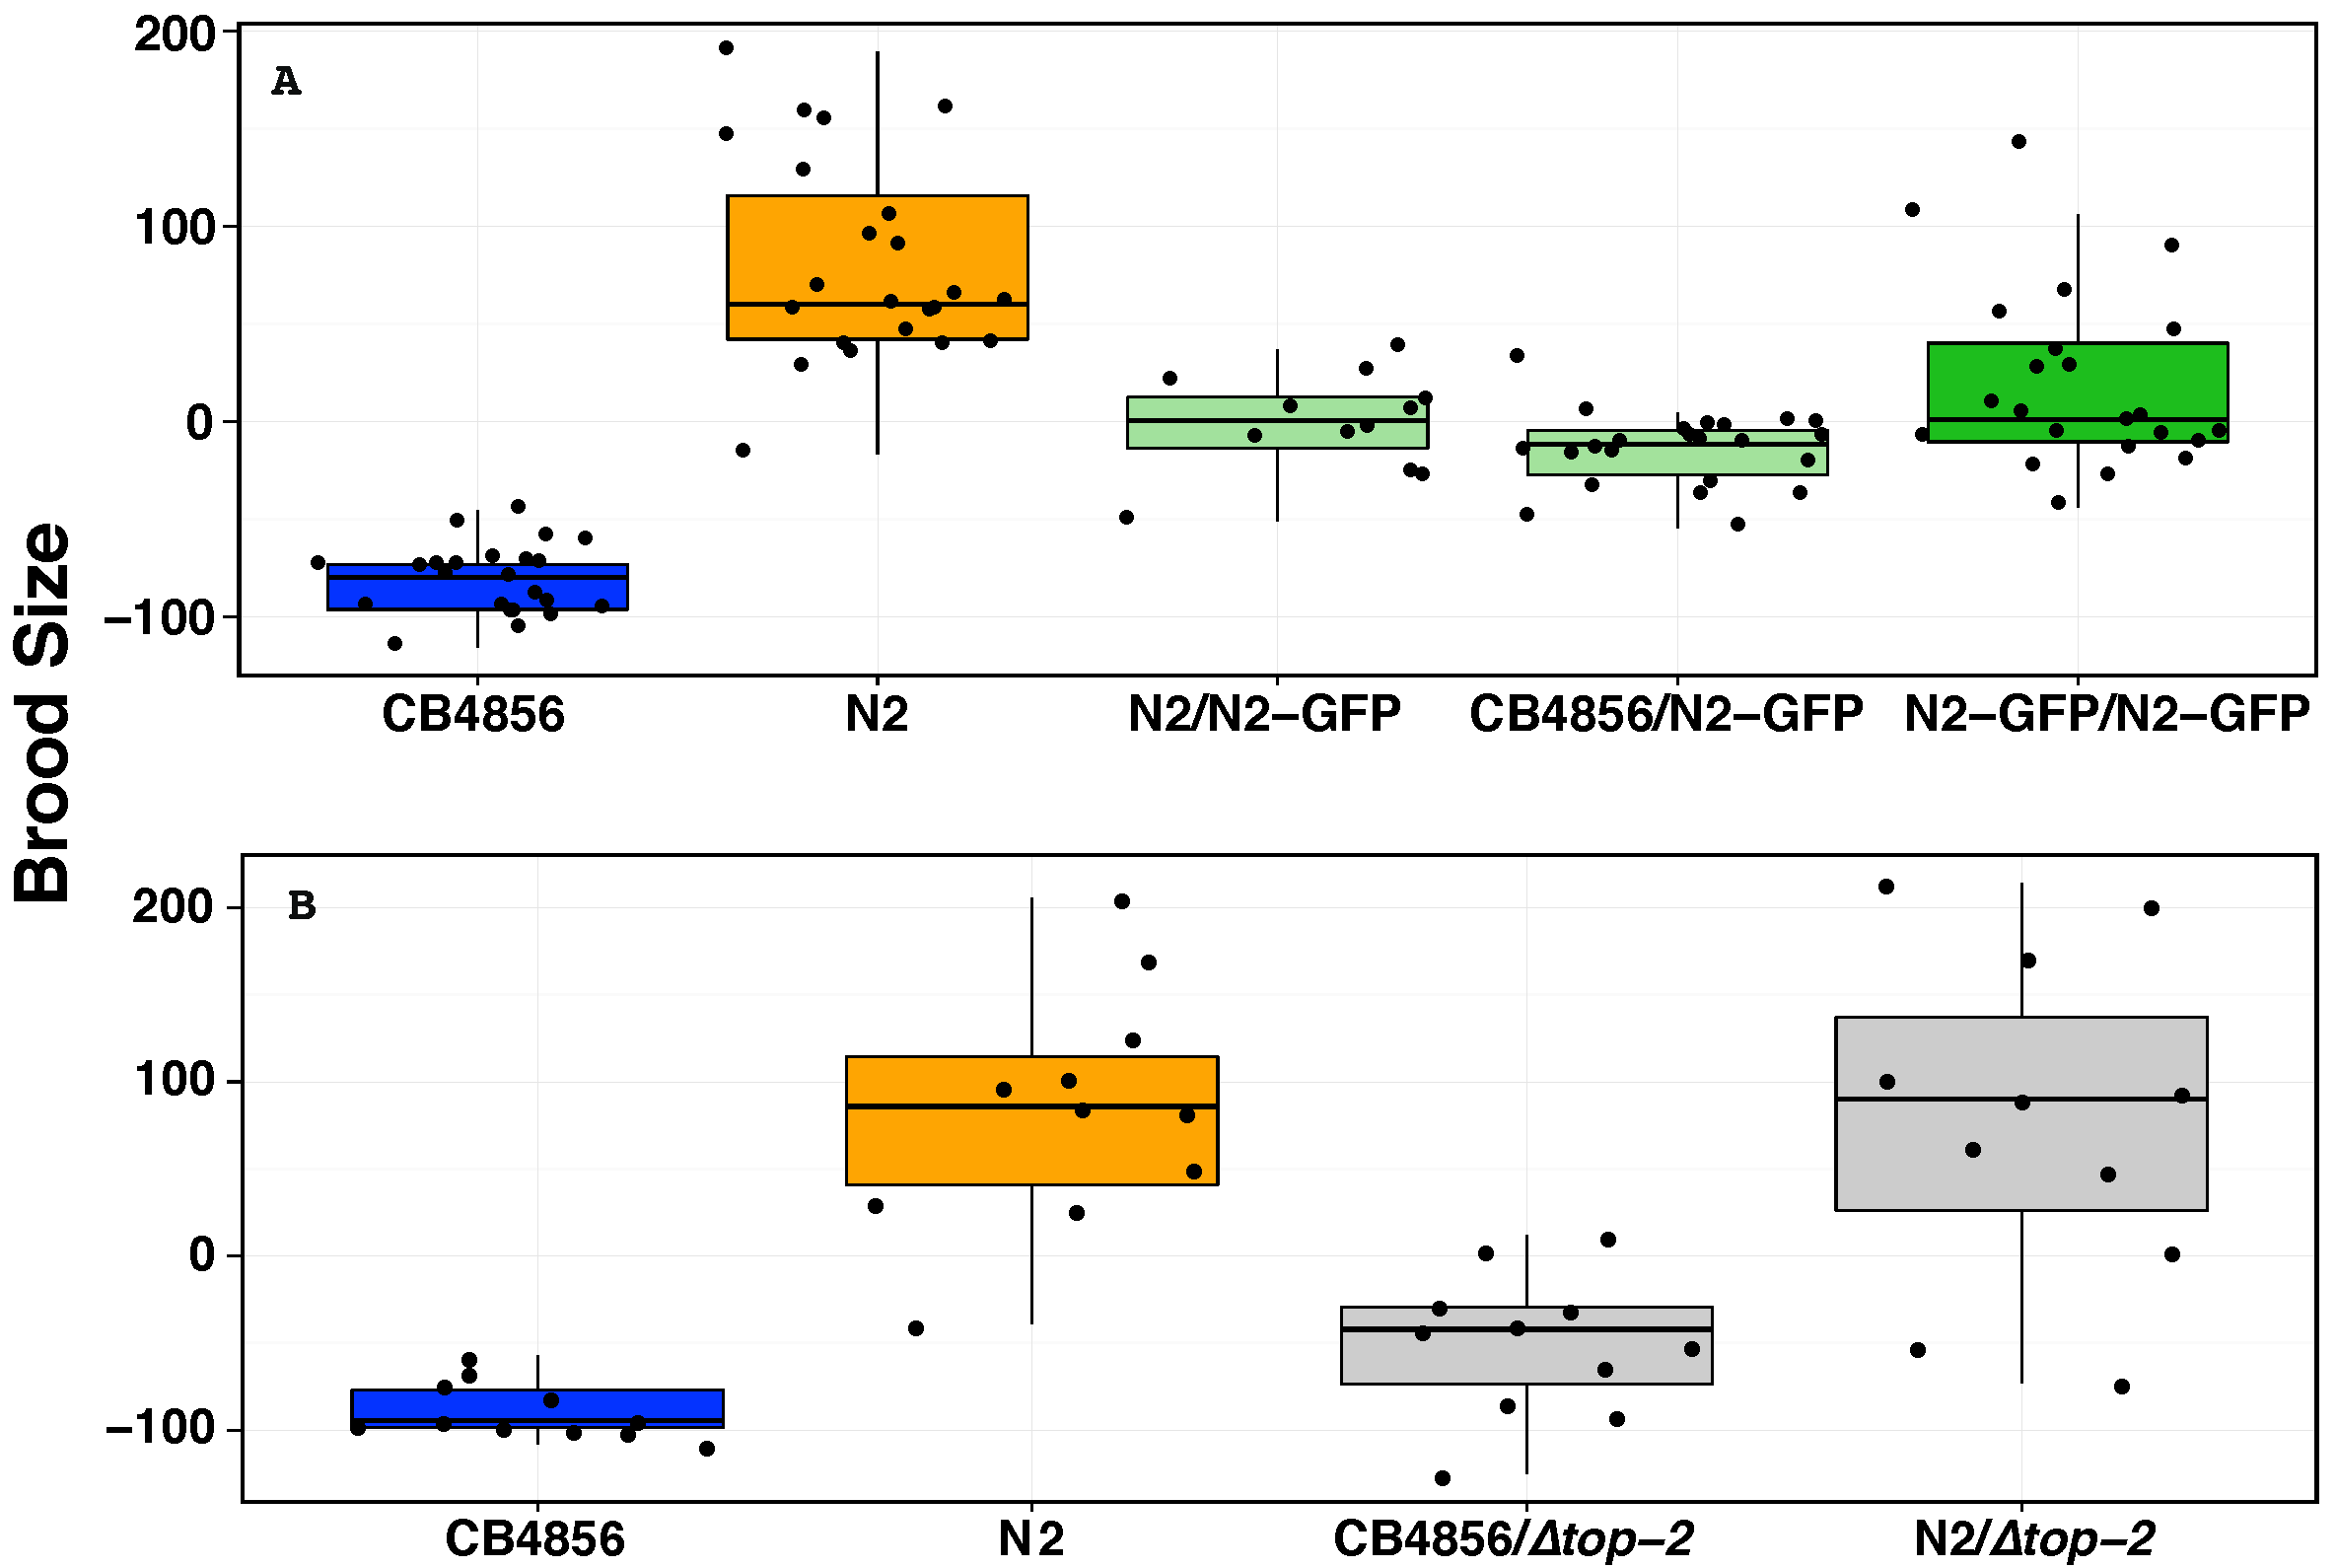
\includegraphics[scale=0.25]{Figures/Figure3.pdf}}
\end{figure}

A traditional test of gene function is the complementation test. In this test, strains with two independently derived mutations with similar homozygous recessive phenotypes are crossed to form heterozygous progeny. If heterozygous animals express the wild-type phenotype, the wild-type copies of the genes being tested complement each other's functions. However, if the heterozygote has a phenotype similar to the individual homozygous mutations, the mutations fail to complement each other and are deficient in the same gene's function~\cite{Hawley:2006gg}. A prerequisite for the complementation test is that the phenotypes being measured are recessive. In the case of etoposide treatment, sensitivity to etoposide is the recessive trait (\autoref{DomComp}A). Having established etoposide sensitivity as the recessive phenotype, we performed a complementation experiment to determine if a {\it top-2} deletion allele in the N2 genetic background is in the same complementation group as the variants present in CB4856 contributing to etoposide sensitivity. In this experiment, the {\it top-2} deletion and variants in CB4856 failed to express the resistant phenotype, suggesting that the variants in CB4856 contributing to sensitivity are present in the {\it top-2} gene. Though these results are encouraging, interpretation of complementation experiments are not straightforward due to potential second-site non-complementation occurring, which is an especially important consideration when performing a complementation test with two highly diverged members of a species with unknown allelic interactions, as is the case for CB4856 and N2. Supporting our results in the CB4856 genetic background, the {\it top-2} deletion in the N2 genetic background failed to complement the resistance phenotype in another sensitive wild isolate, ED3017, that contains the same variants in {\it top-2} as CB4856 but is more closely related to N2 (not shown).

\vspace{5pt}

An alternative approach that is robust to genetic background is the reciprocal hemizygosity test~\cite{Stern:2014jp}. In this test, the same presumptive null mutation is generated in each genetic background ({\it e.g.} null {\it top-2} mutation into CB4856 and N2). Mutants in each genetic background are crossed to the wild-type strain of the other genetic background, thus generating reciprocal hybrids that are genetically identical except for the candidate gene, which is hemizygous. Thus, any difference in the measured phenotypes between reciprocal hybrids can be attributed to the candidate gene being tested. 
\vspace{5pt}

Animals with heterozygous null mutations in candidate genes are needed to perform the reciprocal hemizygosity test. I will generate these strains via CRISPR/Cas mediated genome engineering technique that uses a visible co-conversion marker~\cite{Arribere:2014ku}. This approach depends on the presence of the following factors: 1) an NGG protospacer adjacent motif (PAM) site, 2) the Cas9 endonuclease, 3) small guide RNA (sgRNA) targeting gene of interest, 4) sgRNA targeting co-conversion gene ({\it dpy-10}), 5) {\it dpy-10} repair template (100 nucleotide single-stranded oligonucleotide), and 6) a plasmid repair template that contains an endogenous {\it C.~elegans} promoter driving GFP expression with 50 nucleotide homology arms flanking the cut site. The key aspect to this approach is the nature of the co-conversion marker, {\it dpy-10(cn64)}. {\it dpy-10(cn64)}/+ heterozygotes express a visible roller (Rol) phenotype, {\it dpy-10(cn64)}/{\it dpy-10(cn64)} homozygotes are dumpy (Dpy), and {\it dpy-10(cn64)}/{\it dpy-10(0)} are Dpy and Rol. Being able to identify heterozygous mutants is key because CRISPR/Cas9 mediated cutting typically leads to the generation of heterozygotes. Therefore, heterozygous Rol animals indicate successful injection and expression of all constructs required for genome editing and will serve as an internal control that the system is working. Importantly, when generating allele replacement strains without a visible GFP marker (section \ref{Aim22}), identifying Rol animals substantially reduces the number of offspring that need to be screened by genotyping.
\vspace{5pt}

The experimental flow for generating strains using this approach is outlined in \autoref{CRISPR}. The overall goal is to generate strains with null mutations with a visible marker for easy identification for maintenance and crosses. $P_{0}$ animals are injected with the constructs listed above and transferred to individual plates. Rol {\it dpy-10(cn64)}/+ heterozygous $F_{1}$ progeny are identified and transferred to individual plates and allowed to lay embryos. $F_{2}$ animals from positive plates that do not have the Rol phenotype will be visually inspected for the presence of GFP. Animals with GFP expression will be transferred to new plates and allowed to self. Initial screening for Rol animals is preferred because it does not require a fluorescence microscope and because sgRNA targeting efficacy is highly variable ({\it i.e} the {\it dpy-10} sgRNA is an internal control for editing events)~\cite{Arribere:2014ku}. Essential genes will be maintained as heterozygotes by following the presence of GFP ({\it i.e.} they can not be homozygous for GFP due to lethality, as is the case with the {\it top-2} gene). Genes that are not essential will be allowed to homozygose the null mutation, thus generating a stable stock of the animals. The reciprocal hemizygosity test will then be performed on generated strains. Another advantage of using gene disruption via GFP knock-in is that it reduces the chances of transvection occurring due to disruption of regulatory features. 
\vspace{5pt}

The following description of the reciprocal hemizygosity test will be for the {\it top-2} gene, but a similar approach will be taken for candidate genes identified after NIL generation. N2 {\it\textDelta top-2::GFP}/{\it top-2} animals will be crossed to CB4856 and CB4856 {\it\textDelta top-2::GFP}/{\it top-2} animals will be crossed to N2, thus generating two reciprocal hybrid strains that are hemizygous for {\it top-2}. Hemizygotic $F_{1}$ progeny will be identified on the cross plate by the presence of GFP. Three hemizygotes will then be placed into experimental assay plates containing 500\textmu M etoposide or DMSO and allowed to self over the course of four days. Progeny will then be scored for fitness traits. Progeny will be a mixture of homozygous and heterozygous individuals, which can be separated computationally by the presence of GFP (or GFP fluorescence intensity in the case of non-lethal mutations), as demonstrated in the dominance experiment mentioned above. Any difference in phenotype will be attributed to {\it top-2} because the genetic background of the individuals is identical. 

\vspace{5pt}

{\bf Specific goals: }Due to the limitations of the complementation test mentioned above, I will focus my efforts on performing the reciprocal hemizygosity test for candidate genes identified in Aim 1.1. Constructs containing the {\it dpy-10} sgRNA and Cas9 have already been generated and are available through Addgene~\cite{Arribere:2014ku}. Construction of target gene sgRNAs requires finding a unique PAM site in the gene and ordering a primer that has a priming site on an empty sgRNA vector with a 20 nucleotide tail homologous to the target sequence just upstream of the PAM site. For the homologous repair template, I will construct a 3x-{\it stop}-{\it SL2::GFP} donor plasmid that can easily be adapted for any target gene by altering flanking homology arms. The SL2 5' splice site and upstream Ur element will allow for the translation of GFP despite the presence of upstream stop codons~\cite{McGrath:2009dx}. Generating a gene-specific plasmid will require two gBlocks that have homology to the 3' and 5' of a donor vector and to the gene of interest~\cite{Gibson:2009bc}. sgRNA plasmids will be constructed as needed ({\it i.e.} when candidate genes are identified). The rate limiting step of this aim will be strain construction by microinjection of the constructs. However, the efficiency of genome editing events mediated by the CRISPR/Cas9 system in {\it C. elegans} has significantly improved in the last two years, with homologous recombination events at the target gene occurring in as high as 80\% of $F_{1}$ Rol animals. 

\vspace{5pt}
{\bf Potential issues: }One issue with the reciprocal hemizygosity test is that some null alleles are dominant lethal. If this is the case, heterozygous nulls can not be generated for the test and I will skip the reciprocal hemizygosity test and go straight to the "gold standard" of homologous recombination mediated allele replacement, described in Section~\ref{Aim22}. An additional concern is that genetic background might effect our ability to generate null mutations in candidate genes. For example, a heterozygous null mutation in N2 is viable, but the same mutation is not viable in CB4856. Though observing this phenomenon can open an interesting avenue for further research into the effects of genetic background, it will be an issue for performing the reciprocal hemizygosity test. To get around this issue, I will attempt to generate the null mutation in a different genetic background that contains the same target gene allele. If I run into the same issue, I will move forward with a allele replacement via homologous recombination. 
\vspace{5pt}

Off-target editing events may occur when using CRISPR/Cas9 mediated genome engineering. To date, no papers have been published that report off-target editing events~\cite{Paix:2014eu}. I will minimize off-target editing events by using software that optimizes the design of sgRNA and checks for potential off target homology sites using BLAST~\cite{Hsu:2013kc}. In cases where homologous sequences are present in the genome and unavoidable, we can genotype generated strains for off-target editing events at predicted sites by Sanger sequencing or perform whole-genome sequencing. If off-target sites are identified, successive generations of backcrossing to the parental strain while maintaining the desired allele will remove them from the genetic background. 
\vspace{-5pt}
\subsubsection{Identifying causal genetic variant}\label{Aim22}

I will use CRISPR/Cas9-mediated allele replacement to identify key variants contributing to differential drug susceptibility. Variants to be tested will be prioritized based on the variant's predicted effect ({\it e.g.} non-synonymous tested before synonymous and non-conservative mutations tested before conservative mutations). Additional prioritization can be made by looking at differential expression of candidate genes between CB4856 and N2. These data have already been collected by Rockman {\it et al.} for a panel of RIAILs generated between CB4856 and N2~\cite{Rockman:2010du}. I can probe this data set for expression QTL (eQTL), which are regions of the genome that contain genetic variation contributing to mRNA expression levels. 
\vspace{5pt}

The approach for generating allele replacement strains is similar to the one described above for generating null mutations. The only difference is that instead of a GFP repair plasmid, a single-stranded oligonucleotide will be used. Design considerations for PAM site location and oligonucleotide are as follows. The PAM site should be as close as possible to the site of allele replacement, with most successful PAM sites occurring within 30bp the target allele replacement ~\cite{Arribere:2014ku,Paix:2014eu}. Optimal length of homology arms present on the repair oligonucleotide template ranges from 30-50nt. Additionally, homology arms should directly flank the position of the nucleotides being swapped. The final consideration for repair constructs is to eliminate the PAM site by incorporating a synonymous mutation at the PAM site in order to prevent re-cutting of genomic DNA after homologous recombination mediated repair. 
\vspace{5pt}

Identification of transgenic lines will not rely on visual inspection of a GFP marker, instead I will use PCR amplification followed by restriction enzyme digestion to validate successful editing events. Gene-specific primers flanking the homologous replacement site will be used to genotype $F_{1}$ Rol animals and $F_{2}$ non-Rol animals from positive $F_{1}$ plates. 
\vspace{5pt}

{\bf Potential issues: }An important consideration for homologous recombination-mediated repair using oligonucleotides is the proximity requirement of PAM selection. It may be difficult to find unique PAM sites and sgRNA target sequences if paralogs of a gene interest exist, as is the case for {\it top-2}. This issue can be avoided by using two PAM sites and PCR repair templates as described by Paix {\it et al.}~\cite{Paix:2014eu}, which allows for more flexibility when selecting PAM sites. In this approach, two PAM sites are used to cut genomic DNA and a PCR product is provided for a repair template. The PCR product will have 30-50 nucleotide homology arms immediately flanking the PAM sites and the desired sequence to incorporate between the PAM sites. Off-target editing will be screened for and back-crossed out of generated strains if present.
\vspace{-5pt}
\subsection{Specific Aim 3 $-$ Determine molecular mechanisms
}\label{Aim3}

Determining how genetic changes alter molecular function and subsequently animal physiology is a crucial step toward predicting the effects of a drug. As it is difficult to plan experiments for currently unknown genes, I will focus this section on determining how genetic variation present in {\it top-2} affects its molecular function in response to etoposide.
\vspace{5pt}

It has previously been shown that the half-life of the human TOPOII\textalpha\, DNA cleavage complex (Top2cc) is approximately 5X longer than that of the TOPOII\textbeta\, isoform's~\cite{Bandele:2008df}, though the authors did not speculate as to why this might be the case. The crystal structures of hTOPOII\textalpha\, and hTOPOII\textbeta\, bound to DNA and etoposide revealed drug-interacting residues in the enzyme~\cite{Wu:2011ih,Wendorff:2012dg}. A key interacting residue is Q778 in hTOPOII\textbeta\,, which corresponds to M762 in hTOPOII\textalpha\,~\cite{Wu:2013dia}. The multiple sequence alignment in \autoref{LODplot}C shows that these residues correspond to Q797 in N2, which is resistant to etoposide, and M797 in CB4856, which is sensitive (\autoref{PxG}). The correspondence between the sensitive allele in {\it C. elegans} and hTOPOII\textalpha\, suggests that this residue is contributing to susceptibility. I hypothesize that the non-polar methionine residue is mediating stabilization of the etoposide bound to the topoisomerase and thus stabilizing the Top2cc complex. It should be noted that it is unlikely that endogenous TOPOII function varies between N2 and CB4856 because variation in response to amsacrine treatment, which is another TOPOII poison, does not map to chromosome II where {\it top-2} is located. 

\vspace{5pt}

{\bf Differential etoposide effect on topoisomerase activity {\itshape in vitro}: }Numerous biochemical assays exist to probe the functionality of topoisomerases {\it in vitro}, which are outlined by Nitiss {\it et al.}~\cite{Nitiss:2001fv}. The most suitable assay to directly test my hypothesis is quantifying the Top2cc half life of the two {\it C. elegans} TOPOII alleles. This assay is performed by incubating purified TOPOII with negatively supercoiled DNA until cleavage-ligation equilibrium ($\sim$6 min for hTOPOII) in the presence of 50~\textmu M etoposide~\cite{Bandele:2007ko,Bandele:2008df}. Reaction mixtures are then diluted and mixture aliquots are stopped with SDS, TOPOII is digested with proteinase K, and DNA is purified in a time-dependent manner. Presence of linear DNA is indicative of the presence of Top2cc. The expectation of this assay is that linear DNA will persist for a longer period of time when the reaction mixture contains CB4856 TOPOII with M797 that I hypothesize is stabilizing etoposide binding.

\vspace{5pt}
{\bf Alternative approach: }To directly test etoposide binding to TOPOII, I can perform a competition assay~\cite{Kingma:1999cc}. In this assay, $[^{3}H]$-etoposide is mixed with topoisomerase and placed on nitrocellulose filters. Cold wash buffer is then flowed over the filter and liquid scintillation is used to quantify remaining $[^{3}H]$-etoposide. This assay will be performed with multiple concentrations of $[^{3}H]$-etoposide and with both {\it C. elegans} TOPOII alleles. The expectation is that the binding curve will shift depending on the binding affinity of etoposide to topoisomerase ({\it e.g.} right shifted for CB4856 {\it top-2} allele). 

\vspace{5pt} 






%----------------------------------------------------------------------------------------
%	BIBLIOGRAPHY
%----------------------------------------------------------------------------------------

\newpage

\bibliography{papers} % Use the NIHGrant.bib file for the reference list
\bibliographystyle{plos2015} % Use the custom  bibliography style included with the template

%----------------------------------------------------------------------------------------

\newpage
\section{Appendix}
\setcounter{figure}{0}  

\begin{figure}[h]
\renewcommand{\thefigure}{A.\arabic{figure}}
%\captionsetup{font=tiny}
\floatbox[{\capbeside\thisfloatsetup{capbesideposition={right,top},capbesidewidth=10cm}}]{figure}[\FBwidth]
{\caption[Phenotyping pipeline]{Phenotyping pipeline. Strains are passaged for five consecutive generations to eliminate any transgenerational effects from starvation or other stress. Embryos are prepped by bleach synchronization and allowed to hatch over night to the L1 larval stage, which are subsequently aliquoted to 96-well liquid growth plates and allowed to develop to the L4 larval stage. Three L4 animals are then sorted using the COPAS large-particle sorter to experimental plates containing drug or control. The animals are then grown for four days at 20$^{\circ}$. During this time the animals will mature to adulthood and lay embryos that will subsequently mature. Prior to scoring fitness traits of the resulting progeny, fluorescent microspheres that are the approximate size of bacteria are added to the experimental wells. The amount of beads the animals pump into their body is measured by the COPAS sorter and is a readout of their ability to pump food through their pharynx. After a five minute incubation with the microspheres, animals are treated with azide to straighten their bodies for more accurate length and optical density measurements, and scored. Phenotypic measurements that are measured by the COPAS sorter include 1) brood size, 2) animal length, 3) animal optical density, and 4) animal fluorescence, which is a readout of accumulated microspheres.}\label{Phenotyping}}
{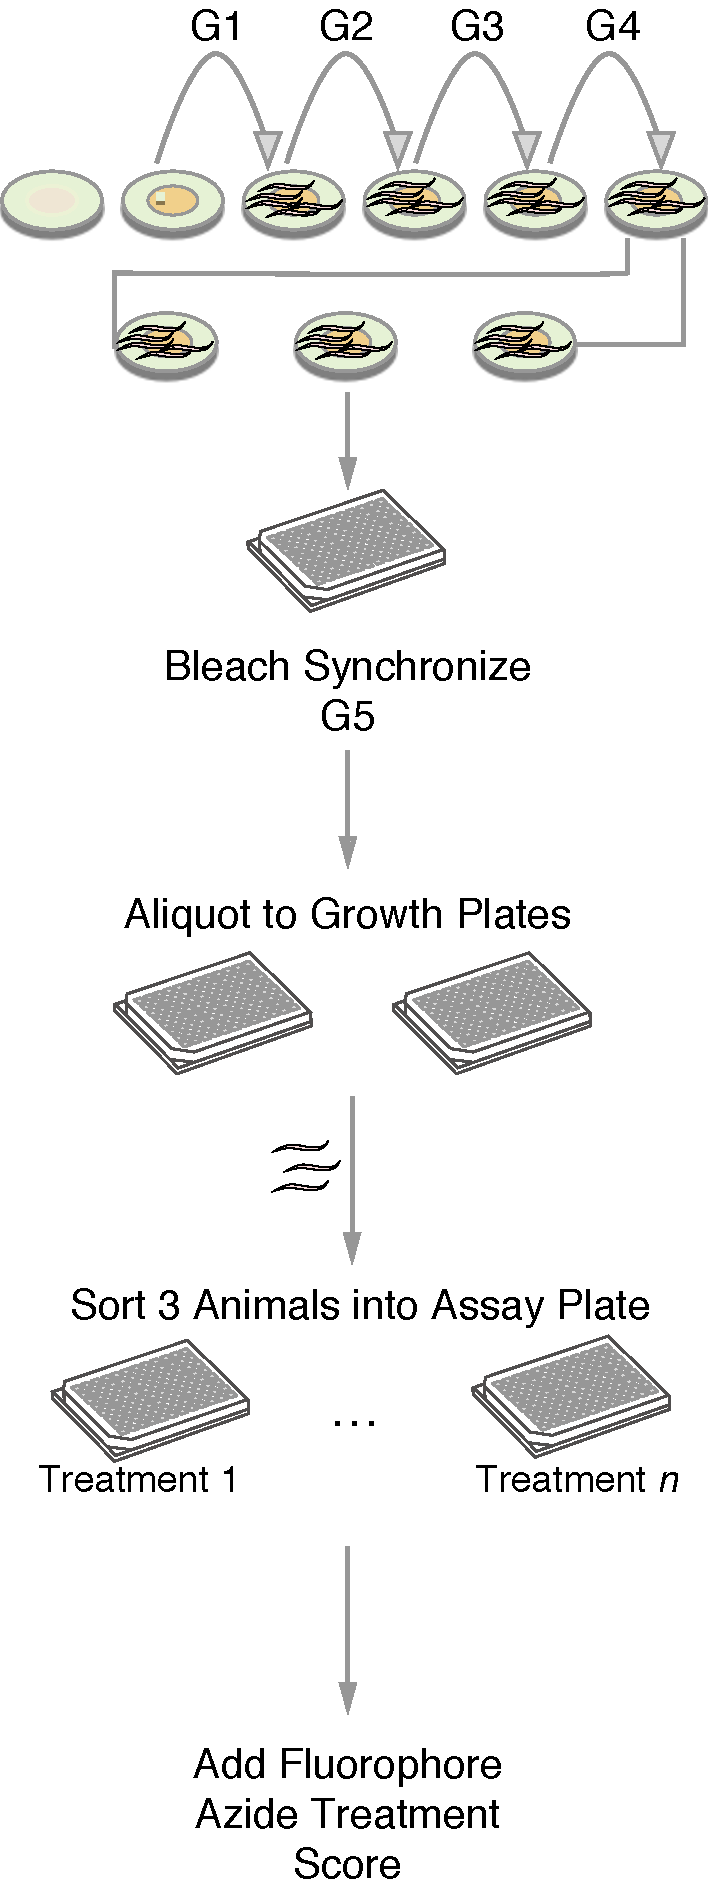
\includegraphics[scale=0.5]{Figures/Appendix_Phenotyping.pdf}}
\end{figure}

\newpage

\begin{figure}[h]
\renewcommand{\thefigure}{A.\arabic{figure}}
%\captionsetup{font=tiny}
\centering
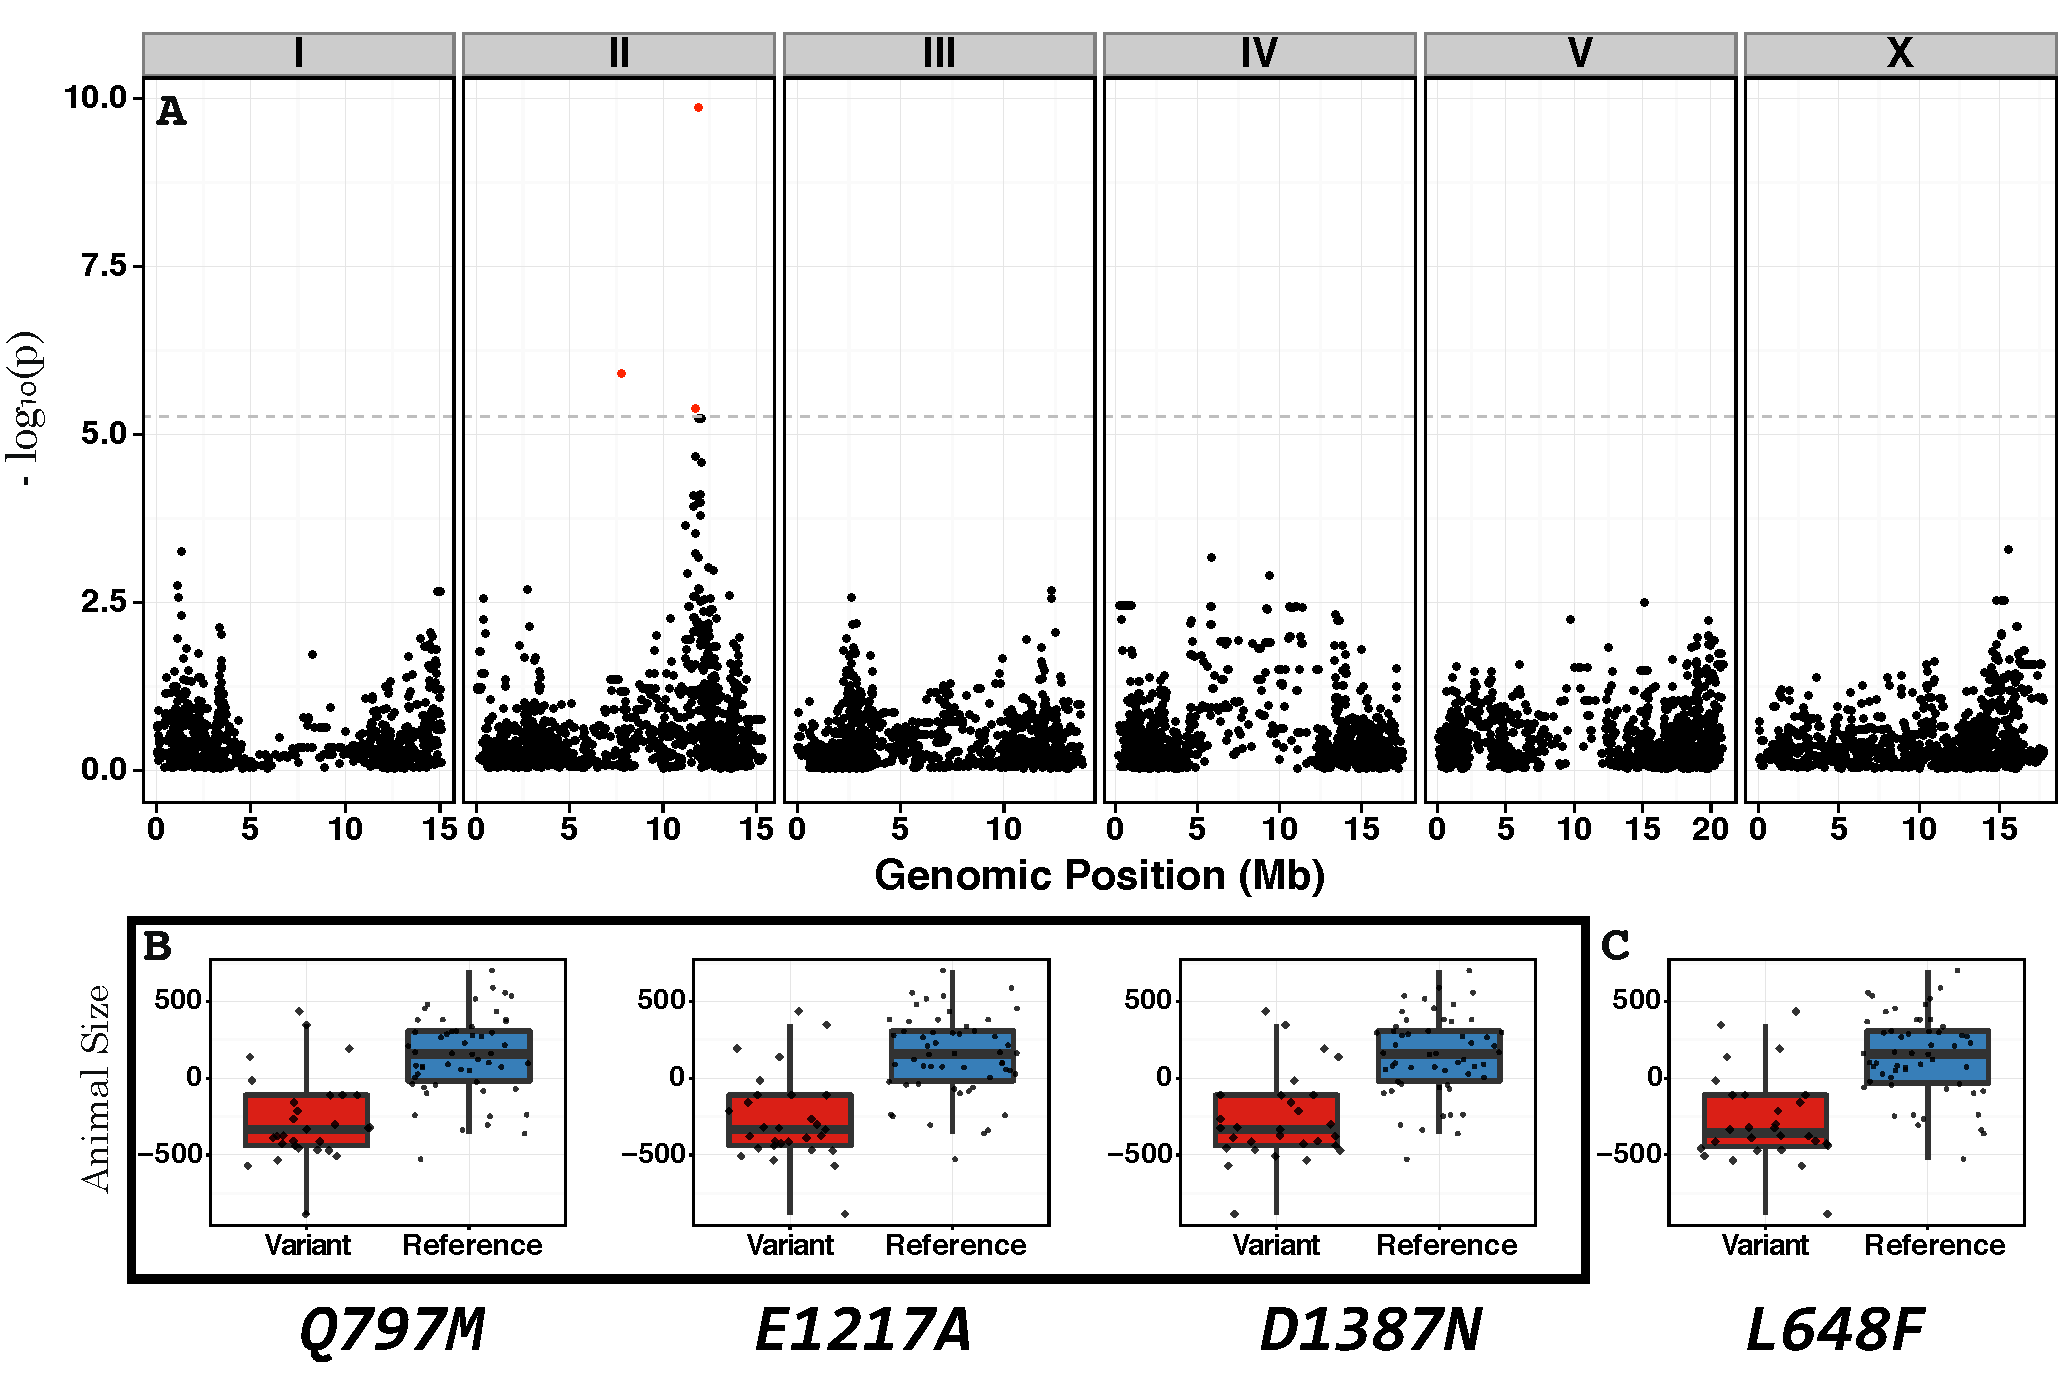
\includegraphics[scale=0.45]{Figures/Appendix_GWAS.pdf}
\vspace{10pt}
\caption[Genome-wide association in response to etoposide]{Genome-wide association in response to etoposide treatment. A) 96 wild {\it C. elegans} isolates were phenotyped using the pipeline described in \autoref{Phenotyping}. Raw data was processed to generate summary statistics, eliminate outliers, and run a genome-wide test for association. Each dot in the figure corresponds to a single-nucleotide polymorphism (SNP). Black dots correspond to SNPs that did not reach Bonferroni-corrected significance levels (indicated by gray dashed line). Red dots correspond to SNPs that did. The peak SNP corresponds to variation present in the {\it top-2} gene. B) Scan for genetic variants highly correlated with phenotypic variation in the QTL confidence interval. This scan was done with the entire SNP set because association mapping was done with a highly pruned SNP set to avoid multiple testing of SNPs in $LD$ blocks. Four of the five variants identified with this approach are in the {\it top-2} gene (three shown in box) and the fifth, L646F, was present in a neighboring gene, {\it npp-3}.}
\label{GWAS}
\end{figure}

\newpage

\begin{figure}[h]
\renewcommand{\thefigure}{A.\arabic{figure}}
%\captionsetup{font=tiny}
\centering
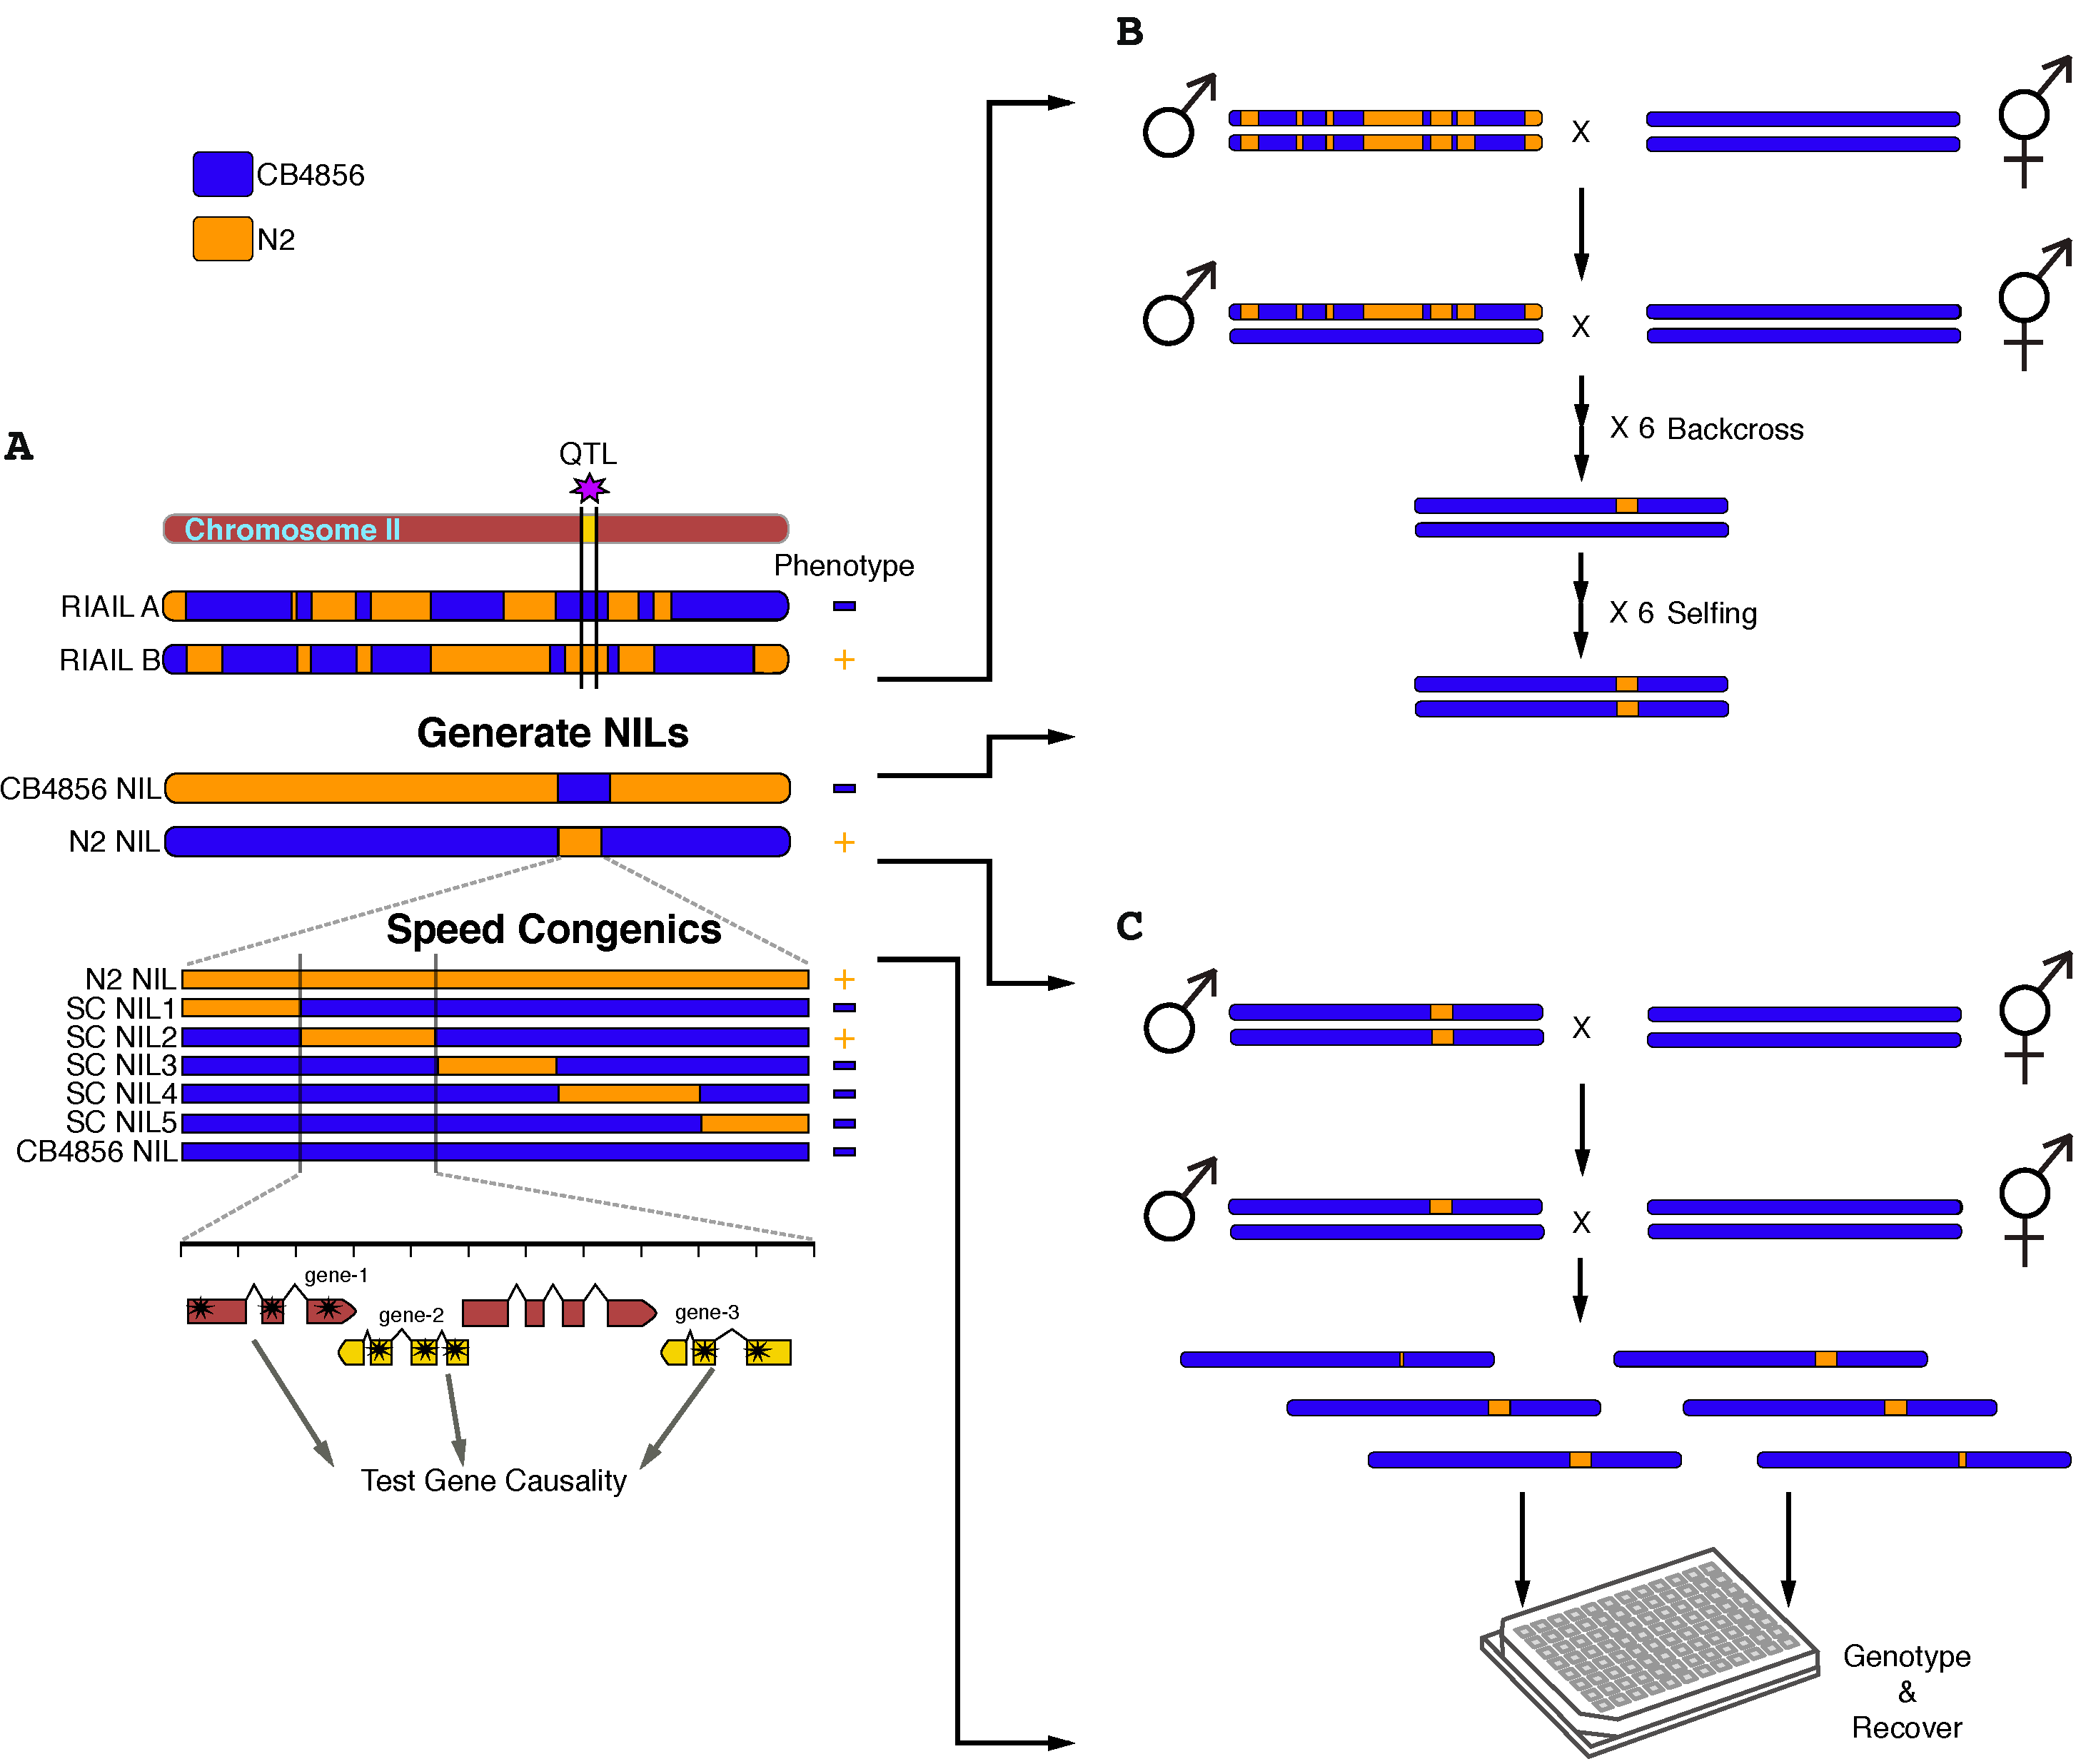
\includegraphics[scale=0.3]{Figures/Appendix_NILs.pdf}
\vspace{10pt}
\caption[Cross designs for NIL generation]{Overview of NIL construction. A) Flow diagram for NIL construction. A QTL (purple star) is identified on chromosome II with a corresponding confidence interval (yellow region on red chromosome). RIAIL strains that contain a single genotype across the entire confidence interval are selected for NIL generation. Generated NILs are then phenotyped to confirm that the introgressed genomic region confers the expected phenotype. NILs are then broken up further using speed congenics and phenotyped. The confidence interval is narrowed down to the genomic region that confers the phenotype of interest, in this case {\bf \textcolor{orange}{+}} refers to resistance. Genes with variants in this region will then be tested for causality. B) Cross design for generating NILs using RIAILs. A male RIAIL that has a single genotype across the confidence interval is crossed to CB4856. Progeny that are males are heterozygotes and are backcrossed to CB4856. Backcrossing is done for six generations to minimize the RIAILs genomic region. Backcrosses are followed by six generations of selfing to homozygous the genome. Genotyping of indels between the strains occurs at every generation. C) Overview of speed congenics. A NIL is backcrossed to CB4856 for two generations. Progeny are then distributed to a single well and allowed to grow. Genotyping is performed on a series of indels across the genomic interval to identify recombinants. Wells that contain recombinants are transferred from wells to agar plates. Individual animals are then distributed to plates and allowed to self and re-genotyped to identify the recombinant progeny. }


\label{NILs}
\end{figure}

\newpage

\begin{figure}[h]
\renewcommand{\thefigure}{A.\arabic{figure}}
%\captionsetup{font=tiny}
\centering
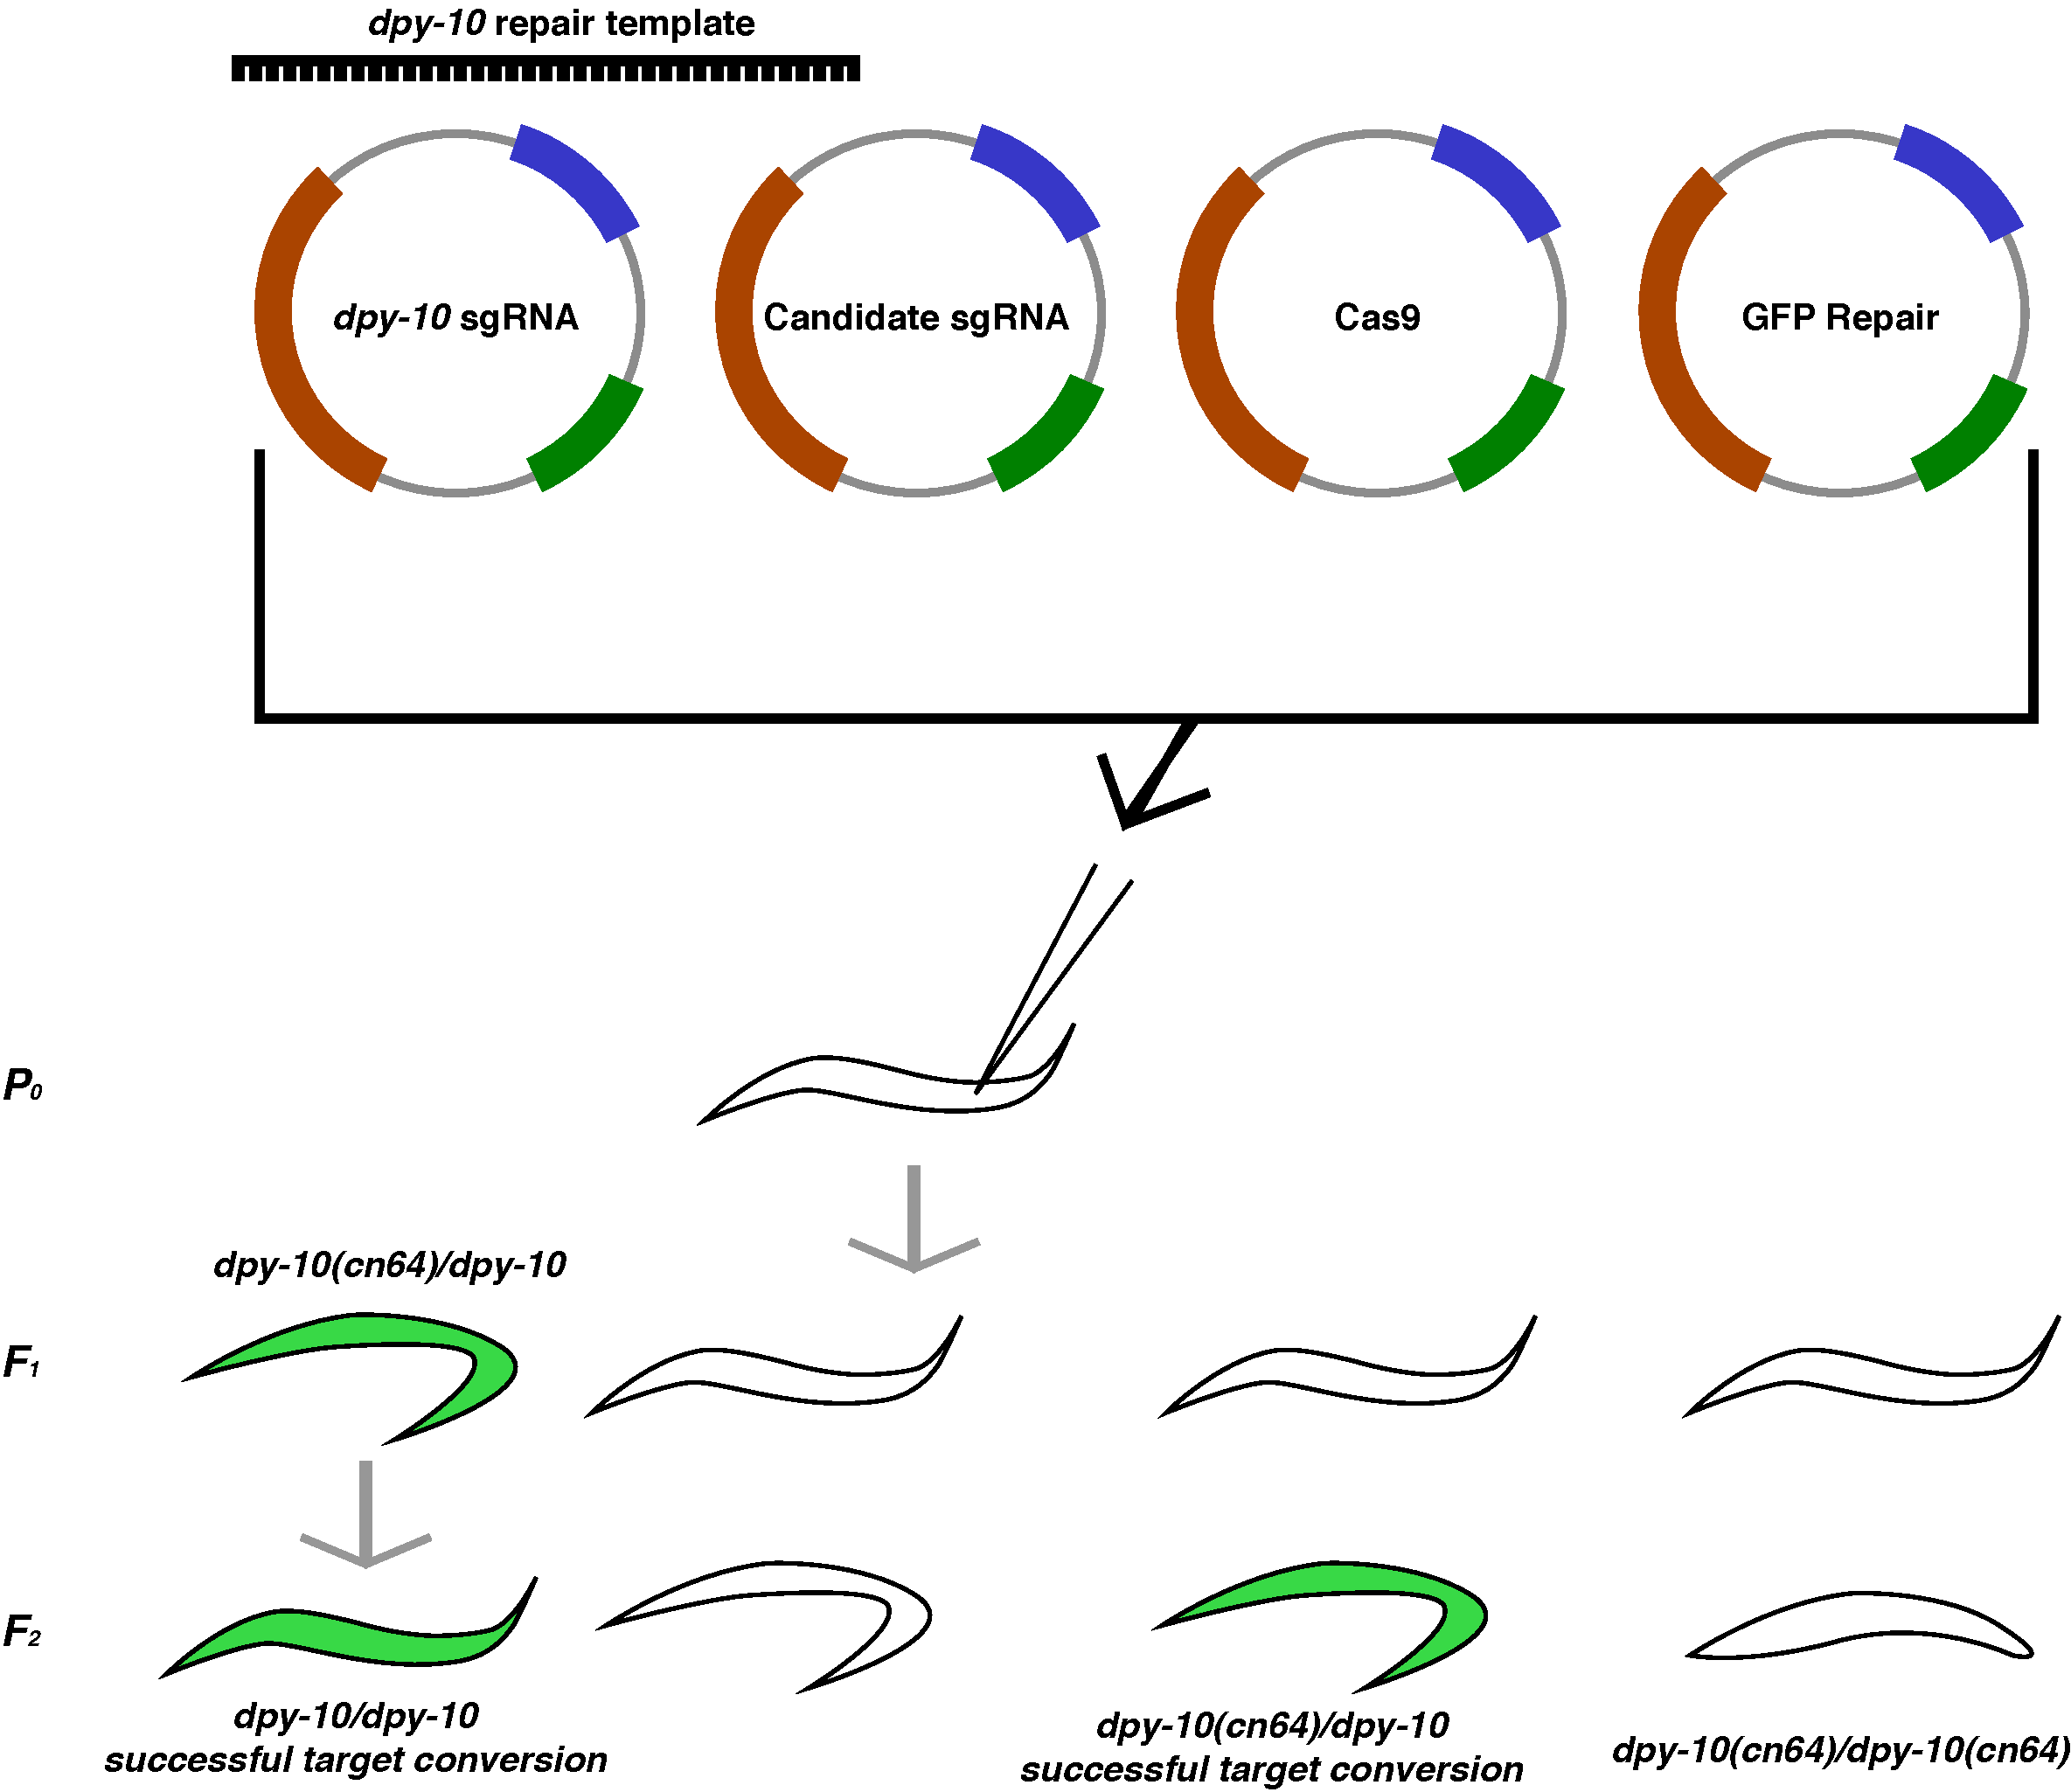
\includegraphics[scale=0.4]{Figures/Appendix_CRISPR.pdf}
\vspace{10pt}
\caption[Overview of CRISPR/Cas mediated genome editing]{Overview of CRISPR/Cas mediated genome editing. Animals are injected in the syncytial gonad with plasmid and oligonucleotide constructs. Injected animals are allowed to lay embryos, which are then allowed to hatch. $F_{1}$ progeny that have the Rol phenotype are identified, transferred to individual plates, and allowed to lay embryos. $F_{1}$ animals are then visually inspected for presence of GFP (or genotyped if performing allele replacement) to identify successful editing events. $F_{2}$ that retain GFP expression and do not have the Rol phenotype are selected.}
\label{CRISPR}
\end{figure}

\newpage

\begin{figure}[h]
\renewcommand{\thefigure}{A.\arabic{figure}}
%\captionsetup{font=tiny}
\centering
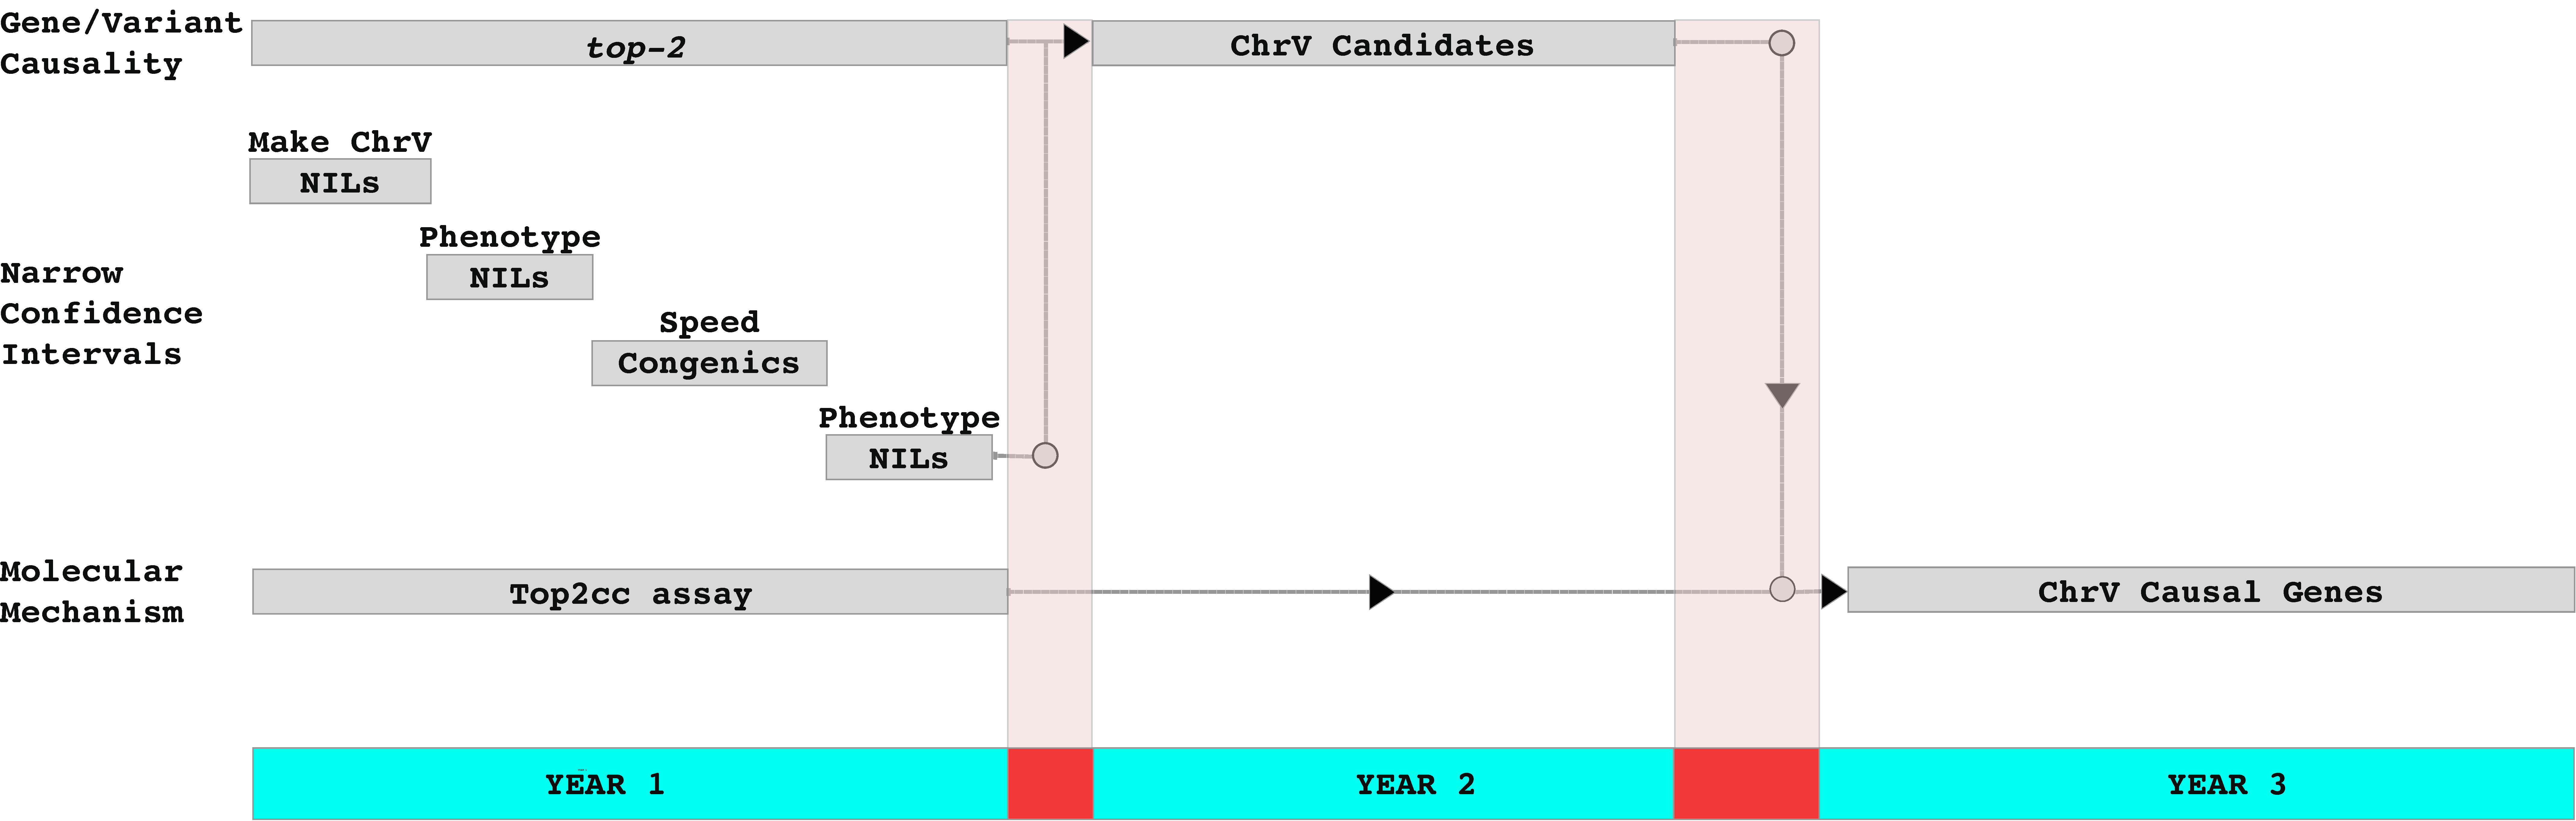
\includegraphics[scale=0.12]{Figures/Appendix_Timeline.pdf}
\vspace{10pt}
\caption[Project Timeline]{Overview of expected timeline for project. Validation of initial results from genetic complementation of the {\it top-2} gene will begin immediately by performing the reciprocal hemizygosity test. I will finish construction of NILs for the chromosome V QTL in response to amsacrine and etoposide and measure disassociation constants for etoposide with each of the TOPOII alleles while construction of chromosome V NILs are being generated. I will perform gene and variant functional tests for candidate genes remaining after NIL construction. Finally, I will perform molecular and biochemical functional tests as new causal variants are discovered.}
\label{Timeline}
\end{figure}

\end{document}